%% LyX 1.6.9 created this file.  For more info, see http://www.lyx.org/.
%% Do not edit unless you really know what you are doing.
\documentclass[oneside,english]{amsart}
%\documentclass[oneside,english]{article}\usepackage[T1]{fontenc}
\usepackage[utf8]{inputenc}
\usepackage{amsmath,amssymb,graphicx}
\usepackage{amsthm}
\usepackage{graphicx}
\usepackage{siunitx}
\usepackage{tikz}
%\usepackage{subfigure}
%\usepackage{epsfig}
%\usepackage{color}
%%%%%%%%%%%%%%%%%%%%%%%%%%%%%%%%%%%%%%%%%%%%%%%%
\graphicspath{{./Images/}}
%usepackage[dvips]{color}
%%%%%%%%%%%%%%%%%%%%%%%%%%%%%%%%%%%%%%%%%%%%%%%%%%%%%
\usepackage[left=2.5cm,right=2.5cm,top=3cm,bottom=3cm]{geometry}
%%%%%%%%%%%%%%%%%%%%%%%%%%%%%%%%%%%%%%%%%%%%%%%%%%%
%\newcommand{\cal}{\mathcal}
\newcommand{\beq}{\begin{equation}}
\newcommand{\eeq}{\end{equation}}
%%%%%%%%%%%%%%%%%%%%%%%%%%%%%%%%%%%%%%%%%%%%%%%%%%%%%
\def\sinc{\mathop{\rm sinc}\nolimits}  
\def\cal{\mathop{\rm cal}\nolimits}  
\def\cal{\mathop{\rm cal}\nolimits}  
\def\CFL{\mathop{\rm CFL}\nolimits}  
\def\VDM{\mathop{\rm VDM}\nolimits}  
\def\RK4{\mathop{\rm RK4}\nolimits}  
\def\ex{\mathop{\rm ex}\nolimits}  
\def\atan{\mathop{\rm atan}\nolimits}  
\def\sech{\mathop{\rm sech}\nolimits}  
\def\tanh{\mathop{\rm tanh}\nolimits}  
\def\div{\mathop{\rm div}\nolimits}  
\def\vort{\mathop{\rm curl}\nolimits}  
\def\vorth{\mathop{\rm curl}\nolimits}  
\def\days{\mathop{\rm days}\nolimits}  
\def\Re{\mathop{\rm Re}\nolimits}  
\def\Sp{\mathop{\rm Sp}\nolimits}  
\newcommand{\bgrad}{\mbox{\boldmath$\nabla$}}
\newcommand{\bnabla}{\mbox{\boldmath$\nabla$}}
\newcommand{\bA}{\mbox{\boldmath$A$}}
\newcommand{\bF}{\mbox{\boldmath$F$}}
\newcommand{\bP}{\mbox{\boldmath$P$}}
\newcommand{\bJ}{\mbox{\boldmath$J$}}
\newcommand{\bM}{\mbox{\boldmath$M$}}
\newcommand{\bg}{\mbox{\boldmath$g$}}
\newcommand{\bq}{\mbox{\boldmath$q$}}
\newcommand{\bx}{\mbox{\boldmath$x$}}
\newcommand{\ba}{\mbox{\boldmath$a$}}
\newcommand{\bb}{\mbox{\boldmath$b$}}
\newcommand{\bc}{\mbox{\boldmath$c$}}
\newcommand{\be}{\mbox{\boldmath$e$}}
\newcommand{\bm}{\mbox{\boldmath$m$}}
\newcommand{\bn}{\mbox{\boldmath$n$}}
\newcommand{\bu}{\mbox{\boldmath$u$}}
\newcommand{\bv}{\mbox{\boldmath$v$}}
\newcommand{\bvv}{\mathbf{v}}
\newcommand{\bgg}{\mathbf{g}}
\newcommand{\bss}{\mathbf{s}}
\newcommand{\bkk}{\mathbf{k}}
\newcommand{\bs}{\mbox{\boldmath$s$}}
\newcommand{\bi}{\mbox{\boldmath$i$}}
\newcommand{\bj}{\mbox{\boldmath$j$}}
%\newcommand{\bJ}{\mbox{\boldmath$J$}}
\newcommand{\bk}{\mbox{\boldmath$k$}}
\newcommand{\bvarphi}{\mbox{\boldmath$\varphi$}}
\newcommand{\bomega}{\mbox{\boldmath$\omega$}}
\newcommand{\bpsi}{\mbox{\boldmath$\psi$}}
%%%%%%%%%%%%%%%%%%%%%%%%%%%%%%%%%%%%%%%%%%%
    \newcommand{\cJ}{\mbox{\mathcal{J}}}
    \newcommand{\fu}{\mathfrak{u}}
    \newcommand{\ftau}{\mathfrak{\tau}}
    \newcommand{\fv}{\mathfrak{v}}
    \newcommand{\fw}{\mathfrak{w}}
    \newcommand{\fz}{\mathfrak{z}}
    \newcommand{\fe}{\mathfrak{e}}
    \newcommand{\fr}{\mathfrak{r}}
    \newcommand{\fg}{\mathfrak{g}}
    \newcommand{\fq}{\mathfrak{q}}
%%%%%%%%%%%%%%%%%%%%%%%%%%%%%%%%%%%%%%%%%%%%%
% ** PERSONAL NEWTHEOREMS
\newtheorem{thm}{Theorem}[section]
\theoremstyle{definition}
\newtheorem{defi}[thm]{Definition}
\newtheorem{prop}[thm]{Proposition}
\newtheorem{coro}[thm]{Corollary}
\theoremstyle{remark}
\newtheorem{remark}[thm]{Remark}

\def\gint{\displaystyle\int}
%\def\vort{\text{vort}}
%\def\vort{\mathop{\rm curl \nolimits}  
%\newcommand{\vort}{\mbox{$\curl_\bn$}}
%\newcommand{\vorth}{\mbox{$\curl_{h,\bn}$}}

%\def\vort{\t}
\usepackage[ruled]{algorithm}
\usepackage{algpseudocode}
\alglanguage{pseudocode}


\makeatother

\usepackage{babel}

\begin{document}

\title{Numerical simulation of propagation problems on the sphere using a compact scheme}

\begin{abstract}
We consider propagation problems on the sphere
and their approximation by finite difference schemes.
The scheme used in this study uses the Cubed Sphere,
a particulra spherical grid with logically Cartesian structure.
A central role is played by the standard one dimensional Hermitian 
derivative. This compact operates in the periodic setting along 
a series of great circles
\cite{Croisille-10, Croisille-12}. 
 Our scheme is centered.
A simple high frequency filter is added to reinforce
the stability. The final scheme is reminiscent of 
compact schemes used in Computational Aeroacoustics or the direct
numerical simulation of turbulence.
% In this paper we consider a compact scheme 
% on the sphere to approximate 
% transport problems,
% a a crucial way the Cubed Sphere grid.
% The scheme is fully centered
% and used a symmetric filter to eliminate high frequency
% oscillating modes. 
Numerical results on a broad series of numerical test cases
in climatology are presented, including
linear convection problems, the linearized shallow water 
and the non linear shallow water equations. 
The results demonstrate the
interest of the present approach 
in a variety of situations arising in numerical climatology.
\end{abstract}

\author{M. Brachet and J.-P. Croisille\dag\ddag}
\address{\dag Universit\'e de Lorraine, D\'epartement de Math\'ematiques, F-57045 Metz, France\\
\ddag C.N.R.S., Institut Elie Cartan de Lorraine, UMR 7502, F-57045 Metz, France}
\email{matthieu.brachet@univ-lorraine.fr, jean-pierre.croisille@univ-lorraine.fr}
\date{February, 21 2018b}
\maketitle
{\sl Keywords: Cubed-Sphere grid - Compact finite difference scheme - 
Hermitian derivative - Vortex propagation}

%% **********************************************************************************************************************************************
\section{Introduction}
\label{sec:1}
In this paper we consider propagation equations on the sphere 
which are of interest in climatology.
The underlying  partial differential equations are related 
to the two dimensional spherical Shallow Water equations (SWE).
The SWE model represents the reference hyperbolic system
to be solved in spherical geometry. 
A second problem (LSWE) consists of the linearized SWE 
around an atmosphere at rest. This problem represents
the basic waves model on the sphere.
It is of fundamental importance 
in climatology and oceanography. On this topic, 
refer to the monograph \cite{Paldor}.

In the past twenty years, the SWE and LSWE systems have been the 
source of many efforts
to adapt conservative methods  
used in numerical gas dynamics.
This is in  particular the case of the finite volume
method \cite{Chen-Xiao, Ullrich-Jablonowski-vanLeer},
or the Discontinuous Galerkin methods \cite{Bao-Nair-Tufo}.

In this paper, we address 
the particular finite difference scheme 
introduced in \cite{Croisille-10,Croisille-12}.
This scheme is compact in the sense of \cite{Collatz,Lele}.
Among the classical methods for fluid flows, it
is strongly related to 
the compact schemes used in computational aeroacoustic
\cite{Visbal-Gaitonde, 
Tam-Webb, Bogey-Bailly} and in turbulence simulation \cite{Kim-Moin}.
The novelty lies in the fact that the approximation
procedure operates on the Cubed Sphere.
Since the scheme is compact, there is the non locality problem
of the finite difference operators. This problem
is traditionnaly handled using one-sided formulas
at near boundary grid points. Here boundary points
are avoided by using a particular set of great circles. 
Overall, our scheme is centered with one value per gridpoint
without staggering.
Finally, a linear high frequency filtering
is added for stabilization purpose. 
In the particular field of numerical climatology, 
our approach can be related to \cite{Arakawa} and more recently
to the compact scheme presented in \cite{Ghader-Nordstrom}.

Three convective models are considered:
\begin{itemize}
\item 
The advection equation: 
\begin{equation}
\label{eq:adv}
\dfrac{\partial h (t,\mathbf{x})}{\partial t}+ \mathbf{c}(t,\mathbf{x}) 
\cdot \nabla_T h(t,\mathbf{x})=0
\end{equation}
The velocity
$\mathbf{c}(t,\mathbf{x})$
% \in \mathbb{T}\mathbb{S}^2$ 
is a prescribed tangential vector field representing the wind.
This linear problem is essential in climatology  
\cite{Williamson-Drake-Hack-Jakob-Swarztrauber}.
The scalar $h(t,x)$ typically 
represents the density of a pollutant convected by the wind with 
velocity $\bc$. 
The numerical solution is compared to 
the analytical solution, which is available by the method of characteristics
and calculable in particular cases.  This permits 
to evaluate, not only the dissipation and the dispersion,
but also to assess the long time behaviour of the scheme.

\item
The linearized Shallow Water model (LSWE) 
\cite{Paldor, Pedlosky} 
%\cite{Paldor, Pedlosky, Vallis} 
linearized at an atmosphere at rest $q_0=[H,\mathbf{v}=\mathbf{0}]$  is
\begin{equation}
\label{eq:lswe}
(LSWE) \left\{
\begin{array}{l}
\dfrac{\partial \eta (t,\mathbf{x})}{\partial t} + H \nabla_T 
\cdot \mathbf{v}(t,\mathbf{x})=S_\eta(t,\bx)\\
\dfrac{\partial \mathbf{v} (t,\mathbf{x}) }{\partial t}+ 
g \nabla_T \eta(t,\mathbf{x}) + f(\mathbf{x}) \mathbf{k}(\mathbf{x}) \times
\mathbf{v}(t,\mathbf{x})=S_{\bv}(t,\bx)\\
\end{array}
\right.
\end{equation}
This system is the basic model for wave problems 
on the sphere since Laplace. It represents the small perturbation
height $\eta$ and velocity $\bvv$.
The source terms $S_\eta$ and $S_{\bvv}$ stand for forcing functions.
The vector function $f \bkk \times \bvv$ represents the Coriolis force.
This wave problem still offers many mathematical open questions \cite{Paldor}.
Accurate numerical simulations are important to get insight in this problem.
\item The full SWE system \cite{Pedlosky} 
in vector form is:\begin{equation}
\label{eq:swe}
(SWE) \left\lbrace
\begin{array}{l}
\dfrac{\partial h^{\star}}{\partial t} (t,\mathbf{x}) + \nabla_T \cdot \left( h^{\star}(t,\mathbf{x}) \mathbf{v}(t,\mathbf{x}) \right) =  0 \\
\dfrac{\partial \mathbf{v}}{\partial t}  (t,\mathbf{x}) + \nabla_T \left( \dfrac{1}{2} |\mathbf{v}(t,\mathbf{x})|^2 
+ g h(t,\mathbf{x}) \right) + \left( f(\mathbf{x}) + \zeta(t,\mathbf{x}) \right) \mathbf{n}(\mathbf{x}) \times \mathbf{v}(t,\mathbf{x}) =  \mathbf{0} 
\end{array}
\right.
\end{equation}
where $\zeta = \left( \nabla_T \times \mathbf{v} \right) \cdot \mathbf{n}$ 
is the {\it relative vorticity} and 
$h^{\star} = h - h_s$ with $h_s$ the bottom topography function.
\end{itemize}
For these three models, and for the test cases considered,
we show that our centered compact scheme compares 
favourably with traditional conservative upwind methods,
such as the finite volume method \cite{Ullrich-Jablonowski-vanLeer}
or the Discontinuous Galerkin method \cite{Nair-Choi-Tufo,Bao-Nair-Tufo}.
The numerical diffusion in our case relies on a
simple linear filtering.
Therefore our scheme is similar in the principle
to approximation procedures for wave models.
As we shall see this scheme with a somewhat
linear design is sufficient to handle
without any nonlinear treatment
to handle reference test cases.
Since our scheme is a priori not conservative,
we carefully evaluate how evolve the integral values
that are preserved at the continuous level.
Conserd quantities are of two kinds.
There is first the primary conservative quantities,
which are by construction preserved by conservative methods.
For (\ref{eq:swe}) this is here mass and the total energy.
However {\sl derived} quantities such as the relative vorticity or 
the potential enstrophy are 
equally important to conserve. 
Note tyhat there is no guarantee that traditional 
conservative methods actually preserve such quantities. In fact, it is well
known that finite volume schemes can dissipate
vorticity for large times.
This is why we numerically analyze the conservation
properties of our scheme
as a whole, without distinction between primary quantities
and derived quantities.
As we shall see, our scheme performs well
regarding conservation for all these integral quantities.

The outline of the paper is as follows.
In Section \ref{sec:2}, we recall the background of 
our approach along the lines 
of \cite{Croisille-10, Croisille-12}. 
In particular we give the details of the centered approximation
of the gradient, the divergence and the vorticity.
In Sec \ref{sec:num}, we present 
numerical results on a series of test cases
involving (\ref{eq:adv}), (\ref{eq:lswe}) and (\ref{eq:swe}). 
Finally, in Section \ref{sec:annexes}
some analysis of the basic compact scheme is carried out on the 
model of the linear advection equation with periodic setting.
This includes
a convergence analysis of the standard fourth order compact scheme 
as well as the stablity matrix analysis of the fully 
discrete scheme, including filtering.
%%%%%%%%%%%%%%%%%%%%%%%%%%%%%%%%%%%%%%%%%%%%%%%%%%%%%%%%%%%%%%%%%
\section{Numerical scheme using central compact differencing 
on the Cubed Sphere}
\label{sec:2}
In this section, we review the basic of our compact scheme.
This scheme uses a particular property of the Cubed Sphere,
the fact that coordinate lines are great circles sections.
These great circles are used
as a support 
for a particular compact scheme.
Here we use the standard
fourth order Hermitian scheme.
This approach allows to evaluate 
accurate versions of the gradient, the divergence and the vorticity.
%% ********************************************************
\subsection{The Cubed Sphere}
\label{sec:CS}
The Cubed Sphere \cite{Sadourny} is a spherical grid widely used
in numerical climatology.
A modern presentation was given in
\cite{Ronchi-Iacono-Paolucci}.
It is composed of six panels 
labelled with index 
$k=(I), (II), (III), (IV), (V)$ and $(VI)$. Each panel 
matches the face of a cube and
supports a Cartesian grid of size $(N+1)\times (N+1)$.
The integer $N$ represents the spatial resolution.
Each panel is equipped with a 
coordinate system $(\xi,\eta)$.
This coordinate system consists of the two angles
measured along the two "equatorial" great circles 
intersecting at the center of the panel.
The Cubed Sphere is represented on Fig. \ref{fig:1}
and a typical panel is shown
on Fig. \ref{fig:2}.
%%%%%%%%%%%%%%%%%%%%%%%%%%%%%%%%%%%%%%%%%%%%%%%%%%%%%%%%%%%%%%%%
\begin{figure}
\includegraphics[scale=0.4]{Images/fig6.jpg}
\caption{
The Cubed Sphere with resolution parameter $N=16$.
The number of gridpoints is $6 N^2+2$, ($1538$ in this case).
The four panels $(I)$, $(II)$, $(III)$ and $(IV)$ are located
around the equatorial plane $z=0$. 
The indices of the north and south panels are $(V)$ 
and $(VI)$ respectively. 
}
\label{fig:1}
\end{figure}
%%%%%%%%%%%%%%%%%%%%%%%%%%%%%%%%%%%%%%%%%%%%%%%%%%%%%%
\begin{figure}
   \def\svgwidth{0.3 \textwidth}
\input{drawing13.pdf_tex}
\caption{
Frontal view of a panel. 
The points of a typical panel of the Cubed-Sphere are 
classified in three categories:
(i) $(N-1)^2$ circles correspond to the {\sl internal} points; 
(ii) $4 (N-1)$ squares 
correspond to the {\sl edge} points ;
(iii) $4$ pentagons correspond to the {\sl corner} points}
\label{fig:2}
\end{figure}
%%%%%%%%%%%%%%%%%%%%%%%%%%%%%%%%%%%%%%%%%%%%%%%%%%%%%%
The points on panel $k$ are denoted 
$\mathbf{s}_{i,j}^{k}$.
The integer $i$ (resp. $j$) 
denotes the index in the $\xi$ direction (resp. $\eta$) direction.
Our finite difference scheme uses discrete unknowns
at points $\mathbf{s}^{k}_{i,j}$ where $ -N/2 \leq i,j\leq N/2$
and $(I) \leq k \leq (VI)$.
%%%%%%%%%%%%%%%%%%%%%%%%%%%%%%%%%%%%%%%%%%%%%%%%%%%
\subsection{Great circles on the Cubed Sphere}
\label{sec:der_cs}
The spatial approximation used in this paper is based on the standard 
Hermitian derivative.
The Hermitian derivative $\delta_x^H u_j$ is 
obtained by solving the tridiagonal system
\beq
\label{eq:812.45}
\frac{1}{6}\delta^H_x u_{j-1}+
\frac{2}{3}\delta^H_x u_j+
\frac{1}{6}\delta^H_x u_{j+1}
=\frac{u_{j+1}-u_{j-1}}{2 \Delta x}.
\eeq
The truncation error for $\delta^H_x u_j$
satifies
\beq
\label{eq:18.312}
\delta_x^H u_{j}-u^\prime(x_j)=-\frac{1}{180}h^4 u^{(5)}(x_j)+ O(h^6).
\eeq
Here, the main idea consists
in using (\ref{eq:812.45}) along a particular set of great circles
on the Cubed Sphere. This set is defined hereafter.
This permits
to approximate with high accuracy 
the gradient, the divergence and the 
vorticity on the sphere.
This is suggested by the fact that
coordinate lines are great circle sections.
%Two typical such great circles are represented
%in Fig. \ref{fig:patron cs}.
%%%%%%%%%%%%%%%%%%%%%%%%%%%%%%%%%%%%%%%%%%%%%%%%%%%%%
\begin{figure}
\begin{center}
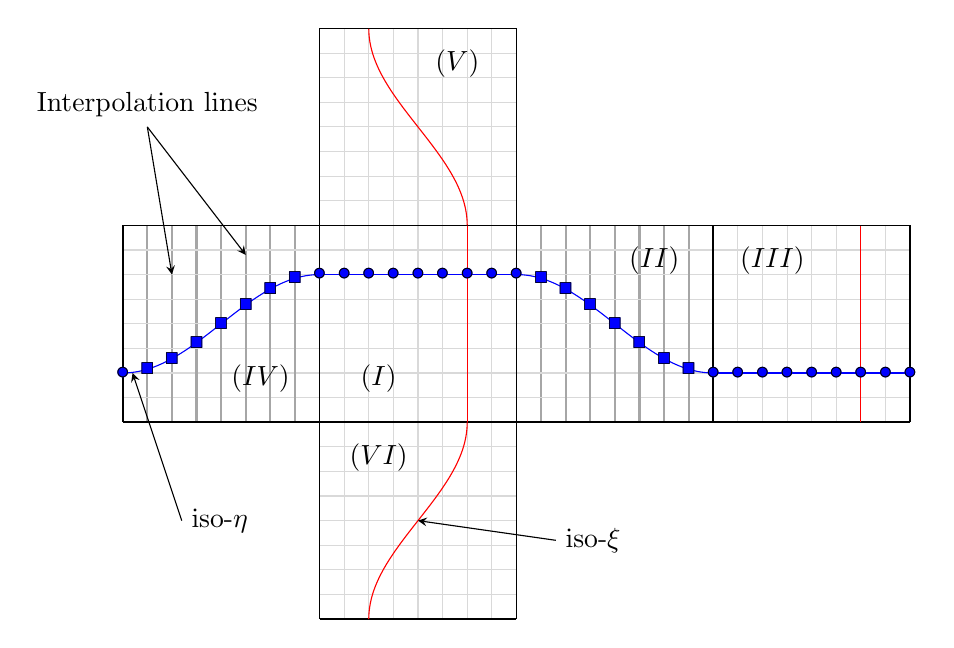
\begin{tikzpicture}[scale=2.5]
	\foreach \x in {1,...,7}
		{ \draw [color=gray!70, line width=0.8pt] (0.125*\x,1) -- (0.125*\x,2) ;
		\draw [color=gray!30] (0,1+0.125*\x) -- (1,1+0.125*\x) ;
		\draw [color=gray!30] (1+0.125*\x,1) -- (1+0.125*\x,2) ;
		\draw [color=gray!30] (1,1+0.125*\x) -- (2,1+0.125*\x) ;
		\draw [color=gray!70, line width=0.8pt] (2+0.125*\x,1) -- (2+0.125*\x,2) ;
		\draw [color=gray!30] (2,1+0.125*\x) -- (3,1+0.125*\x) ;
		\draw [color=gray!30] (3+0.125*\x,1) -- (3+0.125*\x,2) ;
		\draw [color=gray!30] (3,1+0.125*\x) -- (4,1+0.125*\x) ;
		\draw [color=gray!30] (1+0.125*\x,0) -- (1+0.125*\x,1) ;
		\draw [color=gray!30] (1,0.125*\x) -- (2,0.125*\x) ;
		\draw [color=gray!30] (1+0.125*\x,2) -- (1+0.125*\x,3) ;		
		\draw [color=gray!30] (1,2+0.125*\x) -- (2,2+0.125*\x) ;
		}
	

	\draw [line width=0.6pt] (1,3) -- (2,3) ; 
	\draw [line width=0.6pt] (0,2) -- (4,2) ; 	
	\draw [line width=0.6pt] (0,1) -- (4,1) ; 
	\draw [line width=0.6pt] (1,0) -- (2,0) ; 
	
	\draw [line width=0.6pt] (0,2) -- (0,1) ;
	\draw [line width=0.6pt] (1,3) -- (1,0) ;
	\draw [line width=0.6pt] (2,3) -- (2,0) ;
	\draw [line width=0.6pt] (3,2) -- (3,1) ;
	\draw [line width=0.6pt] (4,2) -- (4,1) ; 
	
	\draw (0.7,1.1) node[above]{$(IV)$} ; 
	\draw (1.3,1.1) node[above]{$(I)$} ; 
	\draw (2.7,1.7) node[above]{$(II)$} ;
	\draw (3.3,1.7) node[above]{$(III)$} ;  
	\draw (1.7,2.7) node[above]{$(V)$} ;  
	\draw (1.3,0.7) node[above]{$(VI)$} ; 
	
	\draw [samples=100,domain=0:1,color=blue] plot({\x},{1.5-(2*0.125)*cos(180*\x)});
	\draw [samples=100,domain=1:2,color=blue] plot({\x},{1.5+2*0.125});
	\draw [samples=100,domain=1:2,color=blue] plot({\x+1},{1.5-2*0.125*cos(180*\x)});
	\draw [samples=100,domain=3:4,color=blue] plot({\x},{1.5-2*0.125});
	\draw [>=stealth, <-] (0.05,1.25) -- (0.3,0.5) ;
	\draw  (0.3,0.5) node[right] {iso-$\eta$} ;
	
	\draw [samples=100,domain=0:1,color=red] plot({1.5-2*0.125*cos(180*\x)},{\x});
	\draw [samples=100,domain=1:2,color=red] plot({1.5+2*0.125},{\x});
	\draw [samples=100,domain=1:2,color=red] plot({1.5-2*0.125*cos(180*\x)},{\x+1});
	\draw [samples=100,domain=1:2,color=red] plot({4-+2*0.125},{\x});
	\draw [>=stealth, <-] (1.5,0.5) -- (2.2,0.4) ;
	\draw  (2.2,0.4) node[right] {iso-$\xi$} ;
	
	\draw  (0,1+2*0.125) node[color=blue] {$\bullet$} ;
	\draw (0,1+2*0.125) node {$\circ$} ;
	
	\foreach \k in {0,...,8}
		{\draw  (1+0.125*\k,1.5+2*0.125) node[color=blue] {$\bullet$} ;
	   	\draw (1+0.125*\k,1.5+2*0.125) node {$\circ$} ;
	   	\draw  (3+0.125*\k,1+2*0.125) node[color=blue] {$\bullet$} ;
	   	\draw (3+0.125*\k,1+2*0.125) node {$\circ$} ;
	   	}
	   	
	\foreach \x in {1,...,7}
		{\draw  ({0.125*\x},{1.5-2*0.125*cos(180*0.125*\x)}) node[color=blue] {\begin{tiny}$\blacksquare$\end{tiny}} ;
	   	\draw ({0.125*\x},{1.5-2*0.125*cos(180*0.125*\x)}) node {\begin{tiny}$\square$\end{tiny}} ;
	   	\draw  ({2+0.125*\x},{1.5-2*0.125*cos(180*0.125*\x+180)}) node[color=blue] {\begin{tiny}$\blacksquare$\end{tiny}} ;
	   	\draw  ({2+0.125*\x},{1.5-2*0.125*cos(180*0.125*\x+180)}) node {\begin{tiny}$\square$\end{tiny}} ;
	   	}
	   	
	\draw [>=stealth, <-] (0.25,1.75) -- (0.125,2.5) ;
	\draw [>=stealth, <-] (0.625,1.85) -- (0.125,2.5) ;
	\draw  (0.125,2.5) node[above] {Interpolation lines} ;
\end{tikzpicture}
\caption{Two typical great circles associated to
coordinate lines along the Cubed Sphere.
Periodic compact differencing \ref{eq:812.45} is carried out along each circle,
giving one-dimensional approximate derivatives.
Points marked with circles correspond to 
gridpoints where values are available. In the contrary,
values must be interpolated at points marked with squares.}
\label{fig:patron cs}
\end{center}
\end{figure}
%%%%%%%%%%%%%%%%%%%%%%%%%%%%%%%%%%%%%%%%%%%%%%%%%%%%%%%%%%%%%%%%%%%%%%%
\begin{figure}[htbp]
\begin{center}
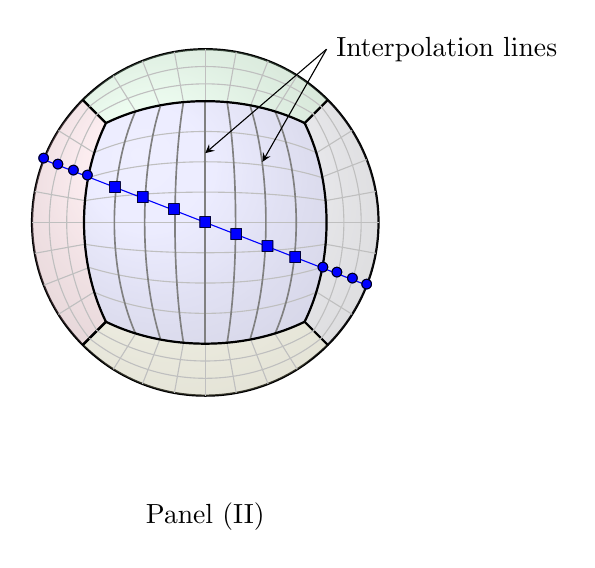
\begin{tikzpicture}[scale=2.2]
	\draw [line width=0.8pt] (0,0) circle (1cm);
    \shade[ball color=blue!10!white,opacity=0.20] (0,0) circle (1cm);	
	
	\filldraw[draw=black,fill=blue!30!white,opacity=0.20]
	plot [smooth,domain=-35:35] ({0.7*cos(\x)},{sin(\x)})
	-- plot [smooth,domain=55:125] ({cos(\x)},{0.7*sin(\x)})
	-- plot [smooth,domain=150:215] ({0.7*cos(\x)},{sin(\x)})
	-- plot [smooth,domain=240:300] ({cos(\x)},{0.7*sin(\x)})
	-- cycle;	
	\draw [samples=100,domain=48:132, color=gray!50] plot({cos(\x)},{0.35*sin(\x)});
	\draw [samples=100,domain=48:132, color=gray!50] plot({cos(\x)},{-.35*sin(\x)});
	\draw [samples=100,domain=46:134, color=gray!50] plot({cos(\x)},{0.175*sin(\x)});
	\draw [samples=100,domain=46:134, color=gray!50] plot({cos(\x)},{-.175*sin(\x)});
	\draw [samples=100,domain=50:130, color=gray!50] plot({cos(\x)},{0.525*sin(\x)});
	\draw [samples=100,domain=50:130, color=gray!50] plot({cos(\x)},{-.525*sin(\x)});
	\draw [samples=100,domain=45:135, color=gray!50] plot({cos(\x)},{0*sin(\x)});

	\draw [rotate=90, samples=100,domain=48:132, color=gray, line width=0.6pt] plot({cos(\x)},{0.35*sin(\x)});
	\draw [rotate=90, samples=100,domain=48:132, color=gray, line width=0.6pt] plot({cos(\x)},{-.35*sin(\x)});
	\draw [rotate=90, samples=100,domain=46:134, color=gray, line width=0.6pt] plot({cos(\x)},{0.175*sin(\x)});
	\draw [rotate=90, samples=100,domain=46:134, color=gray, line width=0.6pt] plot({cos(\x)},{-.175*sin(\x)});
	\draw [rotate=90, samples=100,domain=50:130, color=gray, line width=0.6pt] plot({cos(\x)},{0.525*sin(\x)});
	\draw [rotate=90, samples=100,domain=50:130, color=gray, line width=0.6pt] plot({cos(\x)},{-.525*sin(\x)});
	\draw [rotate=90, samples=100,domain=45:135, color=gray, line width=0.6pt] plot({cos(\x)},{0*sin(\x)});

	\filldraw[draw=black,fill=red!30!white,opacity=0.20]
	plot [smooth,domain=145:215] ({.7*cos(\x)},{sin(\x)})
	-- plot [smooth] (-.573,-.573) -- (-.707,-.707)
	-- plot [smooth,domain=215:145] ({cos(\x)},{sin(\x)})
	-- plot [smooth] (-.707,.707) -- (-.573,.573)
	-- cycle;	
	\draw [line width=0.8pt] (-.573,-.573) -- (-.707,-.707) ;
	\draw [line width=0.8pt] (-.573,.573) -- (-.707,.707) ;
	\draw [color=gray!50] (-.669,.260) -- (-.9321,.3622) ;
	\draw [color=gray!50] (-.669,-.260) -- (-.9321,-.3622) ;
	\draw [color=gray!50] (-.6946,.1259) -- (-.9840,.1783) ;
	\draw [color=gray!50] (-.6946,-.1259) -- (-.9840,-.1783) ;
	\draw [color=gray!50] (-.6427,.4022) -- (-.8477,.5305) ;
	\draw [color=gray!50] (-.6427,-.4022) -- (-.8477,-.5305) ;
	\draw [color=gray!50] (-.707,0) -- (-1,0) ;
	\draw [samples=100,domain=141:219, color=gray!50] plot({0.8*cos(\x)},{sin(\x)});
	\draw [samples=100,domain=138:222, color=gray!50] plot({0.9*cos(\x)},{sin(\x)});
	
	\filldraw[draw=black,fill=green!30!white,opacity=0.20]
	plot [smooth,domain=55:125] ({cos(\x)},{0.7*sin(\x)})
	-- plot [smooth] (-.573,.573) -- (-.707,.707)
	-- plot [smooth,domain=125:55] ({cos(\x)},{sin(\x)})
	-- plot [smooth] (.707,.707) -- (.573,.573)
	-- cycle;	
	\draw [line width=0.8pt] (-.573,.573) -- (-.707,.707) ;
	\draw [line width=0.8pt] (.707,.707) -- (.573,.573) ;
	\draw [rotate=-90,color=gray!50] (-.669,.260) -- (-.9321,.3622) ;
	\draw [rotate=-90,color=gray!50] (-.669,-.260) -- (-.9321,-.3622) ;
	\draw [rotate=-90,color=gray!50] (-.6946,.1259) -- (-.9840,.1783) ;
	\draw [rotate=-90,color=gray!50] (-.6946,-.1259) -- (-.9840,-.1783) ;
	\draw [rotate=-90,color=gray!50] (-.6427,.4022) -- (-.8477,.5305) ;
	\draw [rotate=-90,color=gray!50] (-.6427,-.4022) -- (-.8477,-.5305) ;
	\draw [rotate=-90,color=gray!50] (-.707,0) -- (-1,0) ;
	\draw [rotate=-90,samples=100,domain=141:219, color=gray!50] plot({0.8*cos(\x)},{sin(\x)});
	\draw [rotate=-90,samples=100,domain=138:222, color=gray!50] plot({0.9*cos(\x)},{sin(\x)});
	
	\filldraw[draw=black,fill=yellow!30!white,opacity=0.20]
	plot [smooth,domain=55:125] ({cos(\x)},{-.7*sin(\x)})
	-- plot [smooth] (-.573,-.573) -- (-.707,-.707)
	-- plot [smooth,domain=125:55] ({cos(\x)},{-sin(\x)})
	-- plot [smooth] (.707,-.707) -- (.573,-.573)
	-- cycle;	
	\draw [line width=0.8pt] (-.573,-.573) -- (-.707,-.707) ;
	\draw [line width=0.8pt] (.707,-.707) -- (.573,-.573) ;
	\draw [rotate=90,color=gray!50] (-.669,.260) -- (-.9321,.3622) ;
	\draw [rotate=90,color=gray!50] (-.669,-.260) -- (-.9321,-.3622) ;
	\draw [rotate=90,color=gray!50] (-.6946,.1259) -- (-.9840,.1783) ;
	\draw [rotate=90,color=gray!50] (-.6946,-.1259) -- (-.9840,-.1783) ;
	\draw [rotate=90,color=gray!50] (-.6427,.4022) -- (-.8477,.5305) ;
	\draw [rotate=90,color=gray!50] (-.6427,-.4022) -- (-.8477,-.5305) ;
	\draw [rotate=90,color=gray!50] (-.707,0) -- (-1,0) ;
	\draw [rotate=90,samples=100,domain=141:219, color=gray!50] plot({0.8*cos(\x)},{sin(\x)});
	\draw [rotate=90,samples=100,domain=138:222, color=gray!50] plot({0.9*cos(\x)},{sin(\x)});
	
	\draw [rotate=180,color=gray!50] (-.669,.260) -- (-.9321,.3622) ;
	\draw [rotate=180,color=gray!50] (-.669,-.260) -- (-.9321,-.3622) ;
	\draw [rotate=180,color=gray!50] (-.6946,.1259) -- (-.9840,.1783) ;
	\draw [rotate=180,color=gray!50] (-.6946,-.1259) -- (-.9840,-.1783) ;
	\draw [rotate=180,color=gray!50] (-.6427,.4022) -- (-.8477,.5305) ;
	\draw [rotate=180,color=gray!50] (-.6427,-.4022) -- (-.8477,-.5305) ;
	\draw [rotate=180,color=gray!50] (-.707,0) -- (-1,0) ;
	\draw [rotate=180,samples=100,domain=141:219, color=gray!50] plot({0.8*cos(\x)},{sin(\x)});
	\draw [rotate=180,samples=100,domain=138:222, color=gray!50] plot({0.9*cos(\x)},{sin(\x)});
	
	\draw [samples=100,domain=55:125, line width=0.8pt] plot({cos(\x)},{0.7*sin(\x)});
	\draw [samples=100,domain=55:125, line width=0.8pt] plot({cos(\x)},{-.7*sin(\x)});
	\draw [samples=100,domain=145:215, line width=0.8pt] plot({.7*cos(\x)},{sin(\x)}); 
	\draw [samples=100,domain=145:215, line width=0.8pt] plot({-.7*cos(\x)},{sin(\x)}); 
	
	\draw [color=blue] (-.9321,.3622) -- (.9321,-.3622) ;
	\draw  (-.9321,.3622) node[color=blue] {$\bullet$} ;
	\draw (-.9321,.3622) node {$\circ$} ;	
	\draw  (.9321,-.3622) node[color=blue] {$\bullet$} ;
	\draw (.9321,-.3622) node {$\circ$} ;
	\draw  (-.85,0.3886*.85) node[color=blue] {$\bullet$} ;
	\draw (-.85,0.3886*.85) node {$\circ$} ;	
	\draw (.85,-0.3886*.85) node[color=blue] {$\bullet$} ;
	\draw (.85,-0.3886*.85) node {$\circ$} ;	
	\draw  (-.76,0.3886*.76) node[color=blue] {$\bullet$} ;
	\draw (-.76,0.3886*.76) node {$\circ$} ;	
	\draw (.76,-0.3886*.76) node[color=blue] {$\bullet$} ;
	\draw (.76,-0.3886*.76) node {$\circ$} ;
	\draw  (-.68,0.3886*.68) node[color=blue] {$\bullet$} ;
	\draw (-.68,0.3886*.68) node {$\circ$} ;	
	\draw (.68,-0.3886*.68) node[color=blue] {$\bullet$} ;
	\draw (.68,-0.3886*.68) node {$\circ$} ;	
	\draw (-.52,0.3886*.52) node[color=blue] {\begin{tiny}$\blacksquare$ \end{tiny}} ;
	\draw (-.52,0.3886*.52) node {\begin{tiny}$\square$ \end{tiny}} ;
	\draw (.52,-0.3886*.52) node[color=blue] {\begin{tiny}$\blacksquare$ \end{tiny}} ;
	\draw (.52,-0.3886*.52) node {\begin{tiny}$\square$ \end{tiny}} ;
	\draw (-.36,0.3886*.36) node[color=blue] {\begin{tiny}$\blacksquare$ \end{tiny}} ;
	\draw (-.36,0.3886*.36) node {\begin{tiny}$\square$ \end{tiny}} ;
	\draw (.36,-0.3886*.36) node[color=blue] {\begin{tiny}$\blacksquare$ \end{tiny}} ;
	\draw (.36,-0.3886*.36) node {\begin{tiny}$\square$ \end{tiny}} ;
	\draw (-.18,0.3886*.18) node[color=blue] {\begin{tiny}$\blacksquare$ \end{tiny}} ;
	\draw (-.18,0.3886*.18) node {\begin{tiny}$\square$ \end{tiny}} ;
	\draw (.18,-0.3886*.18) node[color=blue] {\begin{tiny}$\blacksquare$ \end{tiny}} ;
	\draw (.18,-0.3886*.18) node {\begin{tiny}$\square$ \end{tiny}} ;
	\draw (0,0) node[color=blue] {\begin{tiny}$\blacksquare$ \end{tiny}} ;
	\draw (0,0) node {\begin{tiny}$\square$ \end{tiny}} ;
	
	\draw [>=stealth, <-] (.33,.35) -- (.7,1) ;
	\draw [>=stealth, <-] (0,.4) -- (.7,1) ;
	\draw  (0.7,1) node[right] {Interpolation lines} ;
	
	\draw  (0,-1.7) node {Panel (II)} ;

\end{tikzpicture}
\end{center}
\caption{The great circle of Fig. \ref{fig:patron cs}
is shown. The points marked with squares are located on panel (II).
The value assigned to each point is deduced 
by a spline interpolation along each vertical line.
This serves the purpose to evaluate accurately the
derivative along the circle according to the compact formula (\ref{eq:812.45}).}
\label{fig: panel II_interp}
\end{figure}  
%%%%%%%%%%%%%%%%%%%%%%%%%%%%%%%%%%%%%%%%%%%%%%%%%%%%%%%%%%%%%%%%%
Consider for example in Fig. \ref{fig:patron cs}
the great circle crossing panels
$(I),(II),(III)$ and $(IV)$.
This circle coincides with coordinate lines in panels $(I)$ and $(III)$.
In panels $(II)$ and $(IV)$ it does not coincide with
coordinate lines.
Consider now approximating the gradient $\nabla_T f$
of some given function $f$. 
In the sequel $f^\ast$ denotes the restriction 
of $f$ at the grid points.
Thus $(f^\ast)^k_{i,j}$ denotes the
value $f(\bs_{i,j}^k)$.
Based on the values $(f^\ast)^k_{i,j}$ 
one calculates Hermitian derivatives
along this circle. This is operated as follows.
First a suitable set of points $\bm_p$ is defined on this circle.
Second, values $f_p$ are assigned to these points. And third
$\delta^H_x f_{p}$ is calculated using (\ref{eq:812.45}).
Consider the sphere $\Bbb S_a$ with radius $a$.
The Cubed Sphere grid is set up on $\Bbb S_a$ with points
$\bss^k_{i,j}$. 
On each panel $k$, the local basis 
$(\bgg_\xi,\bgg_\eta)$ is
\beq
\label{eq:32.19}
\bgg_\xi(\mathbf{x})=\frac{\partial \mathbf{x}}{\partial \xi},\;\;\;
\bgg_\eta(\mathbf{x})=\frac{\partial \mathbf{x}}{\partial \eta}.
\eeq
Let $f(\bx)$ be a function defined on $\Bbb S_a$.
The gradient of $f(\bx)$ is expressed in terms of the dual basis 
$(\bgg^\xi, \bgg^\eta)$ by
\begin{equation}
\nabla_T f(\bx) = \dfrac{\partial f}{\partial \xi}(\bx) \mathbf{g}^{\xi}(\bx) 
+ \dfrac{\partial f}{\partial \eta}(\bx) \mathbf{g}^{\eta}(\bx)
\label{eq:gradient}
\end{equation}
At $\bss^k_{i,j}$, the two approximate derivatives are used
\beq
\dfrac{\partial f}{\partial \xi}(\bss^k_{i,j}) \simeq \delta^H_\xi f^k_{i,j},\;\;\;
\dfrac{\partial f}{\partial \eta}(\bss^k_{i,j}) \simeq \delta^H_\eta f^k_{i,j}.
\eeq
where the Hermitian derivative $\delta^H_\xi f^k_{i,j}$
and $\delta^H_\eta f^k_{i,j}$ are to be calculated along great circles.
A natural approximate gradient is therefore 
(the subscript $\Delta$ indicate the discrete operator)
\begin{equation}
\nabla_{T,\Delta} (f^\ast)_{i,j}^k 
=\delta^H_\xi (f^\ast)_{i,j}^k \mathbf{g}^{\xi}(\bss^k_{i,j}) 
+\delta^H_\eta (f^\ast)_{i,j}^k \mathbf{g}^{\eta}(\bss^k_{i,j}.
\label{eq:gradient_app}
\end{equation}
where $\delta_\xi^H f^{k}_{i,j}$ and 
$\delta_\eta^H f^{k}_{i,j}$ are evaluated using (\ref{eq:812.45}).
The detailed computational procedure proceeds in four steps
according to Algorithm \ref{algo:41} hereafter. 
Consider again in Fig. \ref{fig:patron cs} the circle 
in horizontal position. This circle corresponds to some 
iso-$\eta$ line $\eta=\eta_0$ in panel (I). The computational 
algorithm \ref{algo:41} 
is applied to all the $\xi$ and $\eta$ 
coordinate lines in panels $(I)$, $(II)$ and $(V)$. 
This is $6 N$ great circles in all, covering the Cubed Sphere. 
We refer to \cite{Croisille-10} for more details.
As a result, the values $\delta^H_{\xi}(f^\ast)^k_{i,j}$ and of 
$\delta^H_{\eta} (f^\ast)^k_{i,j}$ are obtained on the six panels 
and finally the approximation of the gradient is deduced
using (\ref{eq:gradient_app}). In the next section, we 
show how this approach is extended to 
the divergence and the vorticity operators.
\begin{remark}
Observe that the relation (\ref{eq:812.45}) is used with periodic data.
Therefore ghost points or one-sided 
compact operators are never used.
\end{remark}
%%%%%%%%%%%%%%%%%%%%%%%%%%%%%%%%%%%%%%%%%%%%%%%%%%%%%%%%%%%%%%
\subsection{Approximation of differential operators}
\label{sec:op}
In Section \ref{sec:der_cs} we have shown how 
to approximate  the spherical gradient in (\ref{eq:gradient_app}).
Using the same principle, we show how to approximate the divergence and the vorticity.
Consider a tangential vector field
$\bvv(\bx)$. The divergence and curl operators are
expressed in local coordinates as
\beq
\label{eq:95.13.1}
\left\{
\begin{array}{l}
\nabla_T \cdot \bvv= 
\partial_\xi \bvv \cdot  \bgg^\xi +\partial_\eta \bvv \cdot \bgg^\eta,
\;\;(a)\\
\nabla_T \times \bvv = 
\bgg^\xi \times \partial_\xi \bvv + \bgg^\eta \times \partial_\eta \bv
,\;\;(b).
\end{array}
\right.
\eeq
Consider the data $\bvv_{i,j}^{k}$ on the Cubed Sphere.
The discrete divergence and vorticity are defined by 
\beq
\left\{
\begin{array}{l}
\nabla_{T,\Delta} \cdot \bvv_{i,j}^{k}= 
\delta^H_\xi\bvv_{i,j}^{k} \cdot  (\bgg^\xi)_{i,j}^k 
+
\delta^H_\eta\bvv_{i,j}^{k} \cdot  (\bgg^\eta)_{i,j}^k,
\;\;(a), \\
\nabla_{T,\Delta} \times (\bvv)_{i,j}^k = 

(\bgg ^\xi)^k_{i,j}  \times \delta^H_\xi\bvv_{i,j}^{k}
+
(\bgg ^\eta)^k_{i,j}  \times \delta^H_\eta\bvv_{i,j}^{k}
,\;\;(b).
\end{array}
\right.
\label{eq:div_rot}
\eeq
%%%%%%%%%%%%%%%%%%%%%%%%%%%%%%%%%%%%%%%%%%%%%%%%%%%%%%%%%%
\begin{center}
\begin{minipage}[]{12cm}
%\begin{minipage}[H]{12cm}
  \begin{algorithm}[H]
    \caption{: Hermitian derivative along a great circle on the Cubed Sphere}\label{algo:41}
    \begin{algorithmic}[1]
     \State  {\sl Defining the grid on the great circle}. Consider 
a coordinate great circle based on a coordinate line onm panel (I). We set
up a grid of $4 N$ points on this circle (see Fig. \ref{fig:patron cs}) 
$\bm_p$, $p=0,\dots,4N$ with $\bm_0=\bm_{4N}$ as follow:
\begin{enumerate}
	\item The first $N$ points $\bm_p = \bs^{(I)}_{p-N/2,j_0}$, $p=0, ..., N-1$ are located in panel (I). 
They belong to the Cubed Sphere and they carry 
values $u^{(I)}_{p-\frac{N}{2},j_0}$. They are represented by black circles in 
Fig. \ref{fig:patron cs}. 
	\item The next $N$ points $\bm_p$, $p=N...2N-1$ belong to panel (II).
They do not belong to the Cubed Sphere. Values must be interpolated 
at these points. They are represented by black squares 
in Fig. \ref{fig:patron cs}. These points play the role of auxiliary points. 
	\item The next $N$ points $\bm_p = s^{(III)}_{p-N/2,j_0}$, $p=2N, ..., 3N-1$ belong to panel (III). 
They belong to the Cubed Sphere and they carry 
values $u^{(III)}_{i,j_0}$. They are represented by black circles on 
Fig. \ref{fig:patron cs}. 
	\item The last $N$ points $\bm_p$, $p=3N...4N-1$ belong to panel (IV).
They do not belong to the Cubed Sphere. Values must be interpolated 
at these points. They are represented by black squares 
in Fig. \ref{fig:patron cs}. These points play the role of auxiliary points.
\end{enumerate}

	\State {\sl Interpolation step}.
In this step data are interpolated from the Cubed-sphere to the points $\bm_p$:
\begin{enumerate}
\item On panels $(I)$ and $(III)$, the points
marked with black circles belong to the Cubed Sphere. 
Data are just copied
from the Cubed Sphere to the circle. There is no need of interpolation.
\item On panels $(II)$ and $(IV)$, a spline interpolation 
is performed as follows (see \cite{Croisille-10}).
The circle crosses vertical iso$-\xi$ lines. 
A cubic spline interpolation maps the data 
from the vertical iso$-\xi$ line to the points marked with black squares.
This gives a $4$th order interpolation.
\end{enumerate}

	\State {\sl Evaluating the Hermitian derivative on the circle}.
All the points $\bm_p$ now carry values.
The discrete derivative $\delta_{\xi}^H v_p$ is 
evaluated with (\ref{eq:812.45}) using the $v_p$ values given in Step 2. 
This provides $4N$ (periodic) values called $\delta^H_\xi v_p$, $0 \leq p \leq 4N$.
The differentiation is operated with respect to
the equatorial angle. This angle coincides with the $\xi$-coordinate on panel $(I)$ or $(III)$.

	\State {\sl Restricting the approximate derivative to coordinate lines}.
This step consists in retaining the components $\delta^H_\xi v_p$ 
located on panels 
$(I)$ and $(III)$ only . These components are stored. 
They correspond 
to indices $0 \leq p \leq N$ (panel (I)) and $2N \leq p \leq 3N$, (panel (III)).
The values of the derivatives in panels $(II)$ and $(IV)$  
are auxiliary resultsl. They are not stored.

    \end{algorithmic}
    \end{algorithm}
\end{minipage}
\end{center}
%%%%%%%%%%%%%%%%%%%%%%%%%%%%%%%%%%%%%%%%%%%%%%%%%%%%%%%%%%%%%%%
According to \eqref{eq:18.312}, we expect the discrete 
derivatives to be $4$-th. order accurate. 
However, due to the interpolation of the data 
in Step 2 of Algorithm \ref{algo:41}, one may wonder 
if the accuracy could drop to $3$.
In fact, the value $f_p$ assigned to point $\bm_p$ on the circle
satisfies
\beq
\left\{
\begin{array}{l}
f_p = f(\bm_p) \mbox{ if } \bm \mbox { belongs to panels } (I) \mbox { or } (III).\\
f_p = f(\bm_p)+O(\Delta^4) \mbox{ if } \bm  \mbox { belongs to panels } (II) \mbox { or } (IV).
\end{array}
\right.
\eeq
Therefore it turns out that
\begin{equation}
(f_{p+1}-f_{p-1})/(2 \Delta \xi) = (f(\bm_{p+1})-f(\bm_{p-1}))/(2 \Delta \xi)
+O(\Delta ^3),
\end{equation}
which gives in turn
\begin{equation}
\delta_{\xi}^H f_p = \partial_{\xi} f(\bm_p)
+O(\Delta ^3).
\end{equation}
As a consequence the approximations (\ref{eq:gradient_app}), (\ref{eq:95.13.1})$_{a,b}$ are 
at least $O(\Delta ^3)$. In practice however, fourth order accuracy 
has been numerically observed so far.
%%%%%%%%%%%%%%%%%%%%%%%%%%%%%%%%%%%%%%%%%%%%%%%%%%%%%%%%%%%%%%%%%%%%%%%%%%%%%%%%%%%
\subsection{Method of lines}
\label{sec:lines}
Consider as an exemple the SWE system (\ref{eq:swe}).
It is rewritten as
\beq
\partial_t q(t,\bx)=J(q(t,\bx)),
\eeq
where the function $J(q)$ is
\begin{equation}
J(q) = 
\begin{bmatrix}
- \nabla_{T} \cdot \left( h \mathbf{v}\right) \\
- \nabla_{T} \left( \dfrac{1}{2} |\mathbf{v}|^2 
+ g h \right) - \left( f + \zeta  \right) \mathbf{n}  \times \mathbf{v} 
\end{bmatrix}
\end{equation}
According to the method of lines we approximate 
function $F(q)$, and 
then we discretize in time.
The discretization of $F(q)$ is performed 
using the discrete operators \eqref{eq:gradient} and \eqref{eq:div_rot}$_{a,b}$. 
The semi discrete scheme is
\begin{equation}
\label{eq:81.10.8}
\dfrac{d \mathbf{q(t)}}{dt} = J_{\Delta} (\mathbf{q}). 
\end{equation}
where
$\mathbf{q}=[q^k_{i,j}]^T]$ and ${-N/2 \leq i,j \leq N/2}$, $(I) \leq k 
\leq (VI)$. The function $J_\Delta (\mathbf{q})$ is
%%%%%%%%%%%%%%%%%%%%%%%%%%%%%%%%%%%%%%%%%%%%%%%%%%%%%%%%%%
\begin{equation}
\label{eq:76.19}
J_{\Delta}(q) = J_{\Delta}(h_{i,j}^k, \mathbf{v}_{i,j}^k) = 
\begin{bmatrix}
- \nabla_{T,\Delta} \cdot \left( h^{\star k}_{i,j} \mathbf{v}_{i,j}^k \right) \\
- \nabla_{T,\Delta} \left( \dfrac{1}{2} |\mathbf{v}_{i,j}^k|^2 
+ g h_{i,j}^k \right) - \left( f_{i,j}^k + \zeta_{i,j}^k \right) \mathbf{n}_{i,j}^k \times \mathbf{v}_{i,j}^k 
\end{bmatrix}
\end{equation}
where $\zeta_{i,j}^k = \left(\nabla_{T,\Delta} \times \mathbf{v}_{i,j}^k \right) \cdot \mathbf{n}_{i,j}^k$ is the semi discrete relative vorticity. This results in
 The system (\ref{eq:81.10.8}-\ref{eq:76.19}) is a non linear dynamical
system. It is expected to be $4-$th order in $\Delta=\Delta \xi=\Delta \eta$.
There is no upwinding in the approximation in space.
As a consequence, the accuracy of the
discrete equilibrium solutions are 4th order as well.
In particular, the discrete equilibrium is not perturbed by the upwinding
of the flux function in finite volume methods\footnote{
This perturbation requires the so-called well-balanced correction}. 
Refer to Section \ref{sec:4.2.3} for a numerical
example with the SW equations.
As we shall see in the numerical experiments hereafter,
there is no need for additional numerical viscosity in space.
In fact, the intrinsic numerical viscosity of the time scheme,
combined with a linear high frequncy filtering is sufficient
to ensure stability.
%%%%%%%%%%%%%%%%%%%%%%%%%%%%%%%%%%%%%%%%%%%%%%%%
\subsection{Time stepping scheme with filtering}
%%%%%%%%%%%%%%%%%%%%%%%%%%%%%%%%%%%%%%%%%%%%%%%%
\label{sec:13}
The time discretization is based on the classical Runge-Kutta order 4 scheme adding a filtering processus on times by iteration. The time discretization is given by 
Algorithm \ref{alg:RK4F}.
%%%%%%%%%%%%%%%%%%%%%%%%%%%%%%%%%%%%%%%%%%%%%%%%%%%%%%%%%%%%%
\begin{center}
\begin{minipage}[H]{12cm}
  \begin{algorithm}[H]
%\label{algo:4}
    \caption{: Explicit Runge-Kutta Scheme of order 4 with filter}
\label{alg:RK4F}
    \begin{algorithmic}[1]
        \State $q^0 = q^{(0)}$ given
            \For{$n=0,1, \ldots$}
             \State  $K^{(1)} = J_{\Delta} \left( q^n \right)$,
             \State  $K^{(2)} = J_{\Delta} \left( q^n + \dfrac{\Delta t}{2} K^{(1)}\right)$,
             \State  $K^{(3)} = J_{\Delta} \left( q^n + \dfrac{\Delta t}{2} K^{(2)}\right)$,
             \State  $K^{(4)} = J_{\Delta} \left( q^n + \Delta t K^{(3)}\right)$,  
             \State  $q^{n+1} = \mathcal{F} \left( q^n  + \dfrac{\Delta t}{6} \left( K^{(1)} + 2 K^{(2)} + 2 K^{(3)} + K^{(4)} \right) \right)$.
            \EndFor
    \end{algorithmic}
    \end{algorithm}
\end{minipage}
\end{center}
In the 7-th line, $\mathcal{F}$ denotes the so-called {\sl filtering function}.
This filtering step eliminates the +1/-1 mode attached to the grid 
and improves the stability properties (see Section \ref{sec:annexes}).
On the Cubed-Sphere, we use a symmetric filter in the form
\begin{equation}
\mathcal{F} = \dfrac{1}{2} \left( \mathcal{F}_{\xi} \circ \mathcal{F}_{\eta} + \mathcal{F}_{\eta} \circ \mathcal{F}_{\xi} \right).
\end{equation}

Each of the function $\mathcal{F}_\xi$ and
$\mathcal{F}_\eta$ and correspond to a $10$-th
order filter function in the directions $\xi$ and $\eta$ respectively.
We refer to (\ref{eq:75.10.3}), (\ref{eq:11.101}) and 
the last line in Table \ref{tab:filter} 
for the $10$-th order
filter function which is used.
We let operate the filter function $\mathcal{F}_\xi$
along the great circles in a fashion similar to the 
operator $\delta^H_\xi$. In particular,
the steps of the algorithm \ref{algo:41} are identical.
the difference is that the filtering is explicit with a 
non compact stencil.
Two filtering steps are applied at 
each time step to all the components of the
vector $q$. The first one is along the direction $\xi$ 
and the second one 
is along the direction $\eta$.
As in the algorithm \ref{algo:41}, the data are completed 
by an 
interpolation procedure. 
In Section \ref{sec:num}, the $10$-th order filter is used 
both for 
$\mathcal{F}_{\xi}$ and $\mathcal{F}_{\eta}$. 
This has been proved to be a good compromise 
between accuracy and stability.
%We refer to Section \ref{sec:MEA} for the interpretation of 
%the RK4 time stepping  combined with the particular filtering 
%in the case of the linear convection equation.

\begin{remark}
Several variants of compact formulas, of filter functions 
and of interpolation in the interpolation step of Algorithm \ref{algo:41} 
have been tested.
There is no evidence 
of better behaviour or accuracy with alternative choices.
\end{remark}

%%%%%%%%%%%%%%%%%%%%%%%%%%%%%%%%%%%%%%%%%%%%%%%%%%%%%%%%%%%%%%%%%%%%%%%%%%%5
\section{Numerical results}
\label{sec:num}
In this section, we present numerical results obtained 
with our centered compact scheme.
The accuracy of the discrete gradient and divergence
have been analyzed in \cite{Croisille-10, Croisille-12}.
hereafter, we assess the accuracy of the discrete vorticity
on several examples. 
From Section \ref{sec:4.1}, we consider 
the hyperbolic problems (\ref{eq:adv}), (\ref{eq:lswe}) and (\ref{eq:swe}).
In the three cases, the scheme is similar. First the equations
are discretized in space. This gives a system of the form
(\ref{eq:81.10.8}).
Each differential operator 
is applied pointwise at the point of the Cubed Sphere. 
The semi-discrete system (\ref{eq:81.10.8}) is then discretized in time
by Algorithm (\ref{alg:RK4F}). 
Consider a non zero function $f(\bx)$ defined on $\Bbb S_a$. The restriction to
the Cubed Sphere is $(f^\ast)^k_{i,j}=f(\bs^k_{i,j})$. The relative error $e_p$, $p=1,2,\infty$ 
between $f$
and some approximation by $\hat{f}^k_{i,j}$ is
defined by 
\begin{equation}
\label{eq:40.04}
e_p = \frac{\Vert((f^\ast)_{i,j}^{k}) - \hat{f}^k_{i,j} \Vert_p}
{\Vert f^ast_{i,j}^k \Vert_p}
\end{equation}
In (\ref{eq:40.04}), the norm $\Vert . \Vert_p$ stands for
\beq
\Vert f^k_{i,j} \Vert_p= Q(\vert f \vert ^p)^{1/p}
\eeq
where $Q(f)$ stands for 
a discrete integral formula
for grid functions $f^k_{i,j}$.
We have used the rule (20) in \cite{Portelenelle-Croisille})
\beq
\label{eq:87.10.1}
Q(f)= a^2\sum_{k=(I)}^{(VI)} \sum_{i,j=-N/2}^{N/2} c_{i,j} g_{i,j} (f^\ast)^k_{i,j}
\eeq
where the coefficients $g_{i,j}$  and $c_{i,j}$ are given in \cite {Portelenelle-Croisille}.  
%%%%%%%%%%%%%%%%%%%%%%%%%%%%%%%%%%%%%%%%%%%%%%%%%%%%%%%%%%%%%
\subsection{Accuracy of the approximate relative vorticity}
Consider a tangential vector field $\bvv$. 
The {\sl relative vorticity} is denoted by
\begin{equation}
\vort_T (\mathbf{v}) = \left( \nabla_T \times \mathbf{v} \right) \cdot \mathbf{n}.
\end{equation}
We also note $\zeta=\vort_T(\bvv)$.
It is approximated by
\begin{equation}
\label{eq:33.10.3}
\vorth_{T,\Delta}(\mathbf{v}_{i,j}^{k}) = \left( \nabla_{T,\Delta} \times \mathbf{v}_{i,j}^{k} \right) \cdot \mathbf{n}(\mathbf{x}_{i,j}^{k})
\end{equation}
where the discrete curl operator is defined in (\ref{eq:95.13.1}).
We consider some numerical examples 
to asses the accuracy of (\ref{eq:33.10.3}).
In each case, the relative errors $e_p$ in (\ref{eq:40.04}) are reported
associated to the gridfunctions $(\vort_T (\bvv))^\ast$ and the approximation
$\vort_{T,\Delta}(\bvv)$.
%$p=,2$ and $\infty$,
%\begin{equation}
%e_p = \dfrac{\| \vort_{T,\Delta}(\mathbf{v}_{i,j}^{k}) - \vort(\mathbf{v})_{i,j}^{k}  \|_p}{\| \vort(\mathbf{v})_{i,j}^{k}  \|_p}
%\end{equation}
%%%%%%%%%%%%%%%%%%%%%%%%%%%%%%%%%%%%%%%%%%%%%%%%%%%%%%%%%
\begin{enumerate}
\item
The first test consists in assessing the identity
\begin{equation}
\vort_T \left( \nabla_T h \right) = 0.
\label{eq:test3}
\end{equation}
We consider the case
$h(\lambda, \theta) = \cos^5 (\theta) \sin(30 \lambda)$ with $(\lambda, \theta)$ the longitudinal and latitudinal coordinates. The rate accuracy of the scheme is in figure \ref{fig:rate3}. The rate of accuracy is close to $4$ except for $N=8$ because the grid is too coarse. For this test, the error is $\| \vort_{\Delta,T} \left( \nabla_{\Delta,T} h \right) \|_p$ instead of \eqref{eq:40.04}.
\item
%\subsubsection{Test 2 : }
For $\bx=[x,y,z]^T \in \Bbb S^2_a$, the tangential vector 
field is
\begin{equation}
\mathbf{v}(\mathbf{x}) = \mathbf{n}(\mathbf{x}) \times
\begin{bmatrix}
\exp (y/a) \\ \exp (x/a) \\ \exp (z/a)
\end{bmatrix}.
\label{eq:test2}
\end{equation}
The relative vorticity is
\begin{equation}
\vort_T(\bvv)(\bx) 
= \dfrac{1}{a} \mathbf{n}(\mathbf{x}) \times \begin{bmatrix}
-\left( 2 + \frac{z}{a} \right) \exp \left( z/a \right) \\
-\left( 2 + \frac{x}{a} \right) \exp \left( x/a \right) \\
-\left( 2 + \frac{y}{a} \right) \exp \left( y/a \right) 
\end{bmatrix}.
\end{equation}
%%%%%%%%%%%%%%%%%%%%%%%%%%%%%%%%%%%%%%%%%%%%%%%%%%%%%%%%%%%%%%%%%%%%%%%%
\item
The third case represents a zonal wind with velocity
\begin{equation}
\mathbf{v}(\mathbf{x}) = \cos^{\alpha} (\theta) \mathbf{e}_{\lambda}(\mathbf{x}).
\label{eq:test1}
\end{equation}
The relative vorticity is 
\begin{equation}
\vort_T (\mathbf{v})(\mathbf{x}) = \dfrac{\alpha+1}{a} \cos^{\alpha-1} (\theta) \sin (\theta).
\end{equation}
Picking the parameter $\alpha \geq 2$ ensures
that the field and the relative vorticity
are regular near the poles.
We have choosen in our test $\alpha = 3$.
\end{enumerate}
The numerical results for these three tests are similar.
We report in 
Table \ref{tab:rate1} and 
Fig. \ref{fig:rate1} the results for the case 3,
which are typical. 
A sharp fourth order of accuracy can be observed.
This is associated with very good error levels
in the three norms 
$e_p$, for $p=1,2,\infty$.
%%%%%%%%%%%%%%%%%%%%%%%%%%%%%%%%%%%%%%%%%%%%%%%%%%%%%%%%%%%%%%%5
\begin{table}[htbp]
\begin{center}
\begin{tabular}{|c||c|c|c|}
\hline
\textbf{N}  & $\mathbf{e_1}$ & $\mathbf{e_2}$ & $\mathbf{e_{\infty}}$\\
\hline
\hline
$8$  & $2.9158 (-4)$ & $3.3039 (-4)$ & $6.7103 (-4)$ \\
$16$ & $1.7719 (-5)$ & $1.9906 (-5)$ & $4.0648 (-5)$ \\
$32$ & $1.1025 (-6)$ & $1.2416 (-6)$ & $2.5207 (-5)$ \\
$64$ & $6.9056 (-8)$ & $7.7821 (-8)$ & $1.6433 (-7)$ \\
$128$& $4.3244 (-9)$ & $4.8755 (-9)$ & $1.0822 (-8)$ \\
$256$& $2.7061(-10)$ & $3.0522(-10)$ & $6.9474(-10)$ \\
\hline 
\hline
\textbf{Rate}& $4.01$ & $4.01$ & $3.97$\\
\hline
\end{tabular}
\end{center}
\caption{Convergence rate of the approximate relative vorticity 
$\vort_{T,\Delta}(\bvv)$ with $\bvv$ in (\eqref{eq:test1}) with the Hermitian vorticity.}
\label{tab:rate1}
\end{table} 


%%%%%%%%%%%%%%%%%%%%%%%%%%%%%%%%%%%%%%%%%%%%%%%%%%%%%%%%%%%%%%%%%%%%%%%
\begin{figure}
 \begin{minipage}[b]{.46\linewidth}
  \includegraphics[height=5cm]{rate_vort3.png}
  \caption{Convergence rate of the approximate relative vorticity of \eqref{eq:test3} for $e_p$ with $p=1,2$ and $\infty$. $N$ denotes the grid parameter, $N=8$ is a coarse grid. \label{fig:rate3}}
 \end{minipage} \hfill
 \begin{minipage}[b]{.46\linewidth}
  \includegraphics[height=5cm]{rate_vort1.png}
  \caption{Convergence rate of the approximate relative vorticity of \eqref{eq:test1} for $e_p$ with $p=1,2$ and $\infty$ with the same grid parameter than in figure \ref{fig:rate3}. \label{fig:rate1}}
 \end{minipage}
\end{figure}

%%%%%%%%%%%%%%%%%%%%%%%%%%%%%%%%%%%%%%%%%%%%%%%%%%%%%%%%%%%%%%%%
\subsection{Deformational flow with vortices}
\label{sec:4.1}
We consider the convection equation with prescribed velocity
\begin{equation}
\label{eq:adv-2}
\dfrac{\partial h}{\partial t}  (t,\mathbf{x})+ \mathbf{c}(t,\mathbf{x}) 
\cdot \nabla_T h(t,\mathbf{x})=0
\end{equation}
The velocity is prescribed 
to let evolve the initial condition 
with two constant states on a half sphere 
%%into a rollup structure, see Fig. \ref{fig:}.
into a rollup structure.
This structure consists of two vortices localised on two diametraly opposites points $C$ and $C'$. 
As time evolves, filaments
spiral around the vortex center. This behaviour
is well known in point vortex flows.
This test case was introduced in \cite{Nair-Machenhauer, Nair-Jablonowski}
as a sequel of the test case of 
\cite{Williamson-Drake-Hack-Jakob-Swarztrauber}.
Here the analytical solution is available by the characteristics method.
We consider a fixed spatial resolution,
without dynamical adaptivity. 
This case is challenging
to evaluate the spatial accuracy, since
the filaments go below the resolution of the grid at some
time. The time stepping accuracy is also evaluated.
Two variants were introduced in
\cite{Nair-Machenhauer,Nair-Jablonowski}.

In the first variant, the velocity
$\bc(\bx)=c_{\lambda'}(\bx) \be_{\lambda'}(\bx)$ 
(in the coordinate system $(\lambda', \theta')$ 
attached to the axis $(C C^\prime)$) is time independent with
\begin{equation}
\label{eq:34.981}
c_{\lambda'}=\cos(\theta') \omega_r(\theta'),
\end{equation}
where
\begin{equation}
   \omega_r ( \theta') = \left\{ 
   \begin{array}{ll}
      V(\theta')/( a \rho(\theta') ) & \text{ if } \rho \neq 0, \\
      0 & \text{ if } \rho =0.
   \end{array}
   \right.
\label{vitesse_angulaire}
\end{equation}
Let $T>0$, $\rho_0>0 $ and $ v_0 = 2 \pi a / T$
be parameters.
The scalar functions $\rho(\theta')$ and $V(\theta')$ are 
\begin{equation}
\left\{
\begin{array}{l}
\rho(\theta')=\rho_0 \cos(\theta'),\\
V(\theta') = v_0 \dfrac{3 \sqrt{3} }{2} \sech^2 ( \rho(\theta') ) \tanh ( \rho(\theta') ).
\end{array}
\right.
\end{equation} 
The solution $ h(t,\bx)$ is given in coordinates $(\lambda',\theta')$ 
by
\begin{equation}
h(t,\lambda',\theta')=
1 - \tanh \left[ \dfrac{\rho(\theta')}{\gamma} \sin ( \lambda' 
- \omega_r(\theta') t ) \right],
\label{NM_exacte}
\end{equation}
The values 
$\rho_0 = 3$, $ \gamma = 5$ and $T=12$ days 
are used in the computations \cite{Nair-Jablonowski}.
Fig. \ref{fig:57.2} reports 
the error history for $C$ localised in $(\lambda_C, \theta_C) = (\pi/4, \pi/4)$. This corresponds
to a location of the vortices at the intersection
of three panels. This permits to assess 
the accuracy of the gradient calculation with Algorith \ref{algo:41}.
The resolution parameter is $N=36$, which corresponds to
a coarse grid, with equatorial resolution 
of $\Delta \lambda = 2.5 \deg$. 
Two $\CFL = \max_{\mathbf{x} \in \mathbb{S}_a^2}{\mathbf{c}}\Delta t / \Delta \xi$ values were used. In both cases, the scheme
was found stable. For each CFL value, 
the error grows smoothly.
For $\CFL=0.05$ (2880 ite.), the error is dominated by the space approximation.
The observed error levels have the same order of magnitude than 
with the Discontinuous Galerkin method in \cite{Nair-Jablonowski}.
For $\CFL=0.5$ (288 ite.), space and time errors are observed simultaneously.
The error level are slightly better for $\CFL=0.5$ than for 
$\CFL=0.05$. This is a well known effect of the time stepping.
Fig. \ref{table:2.4} reports the convergence rate 
in the norms $p=1$, $p=2$ and $p=\infty$ with $\CFL=0.7$(205 ite.). The error convergence
is of order greater than $4$, which is better than expected.
%%%%%%%%%%%%%%%%%%%%%%%%%%%%%%%%%%%%%%%%%%%%%%%%%%%%%%%%%%%%%%%%%%%%%%%%%%%%%%
\begin{figure}[htbp]
\includegraphics[scale=0.3]{ref_7367656360_normerreur_test_1.png}
\includegraphics[scale=0.3]{ref_7367656531_normerreur_test_1.png}
%\includegraphics[scale=0.4]{ref_7367665245_normerreur_test_1.png}
\caption{Vortex test case of Nair and Machenhauer. 
The axis $(CC^\prime)$ is such that 
$(\lambda_C,  \theta_C) = (\pi / 4, \pi / 4)$.
Grid resolution $N=36$. 
Left panel: error history with $\CFL=0.05$ (2880 ite.). 
Right panel: error history with $\CFL=0.5$ (288 ite.). 
\label{fig:57.2}
}
\end{figure}
%%%%%%%%%%%%%%%%%%%%%%%%%%%%%%%%%%%%%%%%%%%%%%%%%%%%%%%%%%%%%%%%%%%%%%%%%
% \begin{figure}[htbp]
% \includegraphics[scale=0.4]{ref_7367656531_normerreur_test_1.png}
% \includegraphics[scale=0.4]{ref_7367656543_normerreur_test_1.png}
% \caption{Error curves $N=35$; $cfl=0.5$; $(\lambda_P,  \theta_P) 
% = (\pi / 4, \pi / 4)$ (left) and $(\lambda_P, \theta_P) = (0,0)$ 
% (right) for the Nair and Machenhauer test case.}
% \label{erreur_cfl=0.5}
% \end{figure}
%%%%%%%%%%%%%%%%%%%%%%%%%%%%%%%%%%%%%%%%%%%%%%%%%%%%%%%%%%%%%%%%%%%%%%%%%
\begin{figure}[htbp]
\includegraphics[scale=0.5]{rate_NMpi4.png}
\caption{Convergence analysis for the Nair and Machenhauer test case \cite{Nair-Machenhauer}. 
$\CFL = 0.7$ (205 ite.); $(\lambda_C, \theta_C) = (\pi/4,\pi/4)$.}
\label{table:2.4}
\end{figure}

%%%%%%%%%%%%%%%%%%%%%%%%%%%%%%%%%%%%%%%%%%%%%%%%%%%%%%%%%%%%%%%%%%%%%%%%%%%%%
The second variant \cite{Nair-Jablonowski} 
consists in superposing to the preceding velocity a 
solid body rotation at constant speed.
As a result, the rollup behaviour of the two antipodal vortices
is now superposed to the traveling wave effect 
at constant speed. 
This makes the test case even more difficult to handle
for large time. The velocity  $\mathbf{c}(t,\mathbf{x})$ in \eqref{eq:adv} 
is $\mathbf{c}=\mathbf{c}_s +\mathbf{c}_r$
where $\mathbf{c}_s$ is the solid rotation velocity 
\begin{equation}
\left\{
\begin{array}{l}
c_{\lambda, s} = u_0 (\cos \theta \cos \alpha + \sin \theta \cos \lambda \sin \alpha),\\
c_{\theta, s} = -u_0 \sin \lambda \sin \alpha.
\end{array}
\right.
%\label{vitesse_theta_bump}
\end{equation}
$\alpha$ is a rotation parameter. $u_0 = 2 \pi a / T$ with $T$ the simulation time (here, 12 or 24 days).
$\mathbf{c}_r$ is the "static" velocity in (\ref{eq:34.981}).
In (\ref{NM_exacte})
$(\lambda_C, \theta_C)$ is replaced by the solid body 
rotation given  by 
\begin{equation}
(\lambda_s, \theta_s) = (\lambda_0 + w_s t, \theta_0)
\end{equation}
where $(\lambda_0, \theta_0) = (3 \pi /2, 0)$ is the initial position of the vortex.
On the other hand, the solid-body velocity is given by
\begin{equation}
\left\{
\begin{array}{l}
c_{\lambda, r} = a \omega_s \left( \sin \theta_C(t) \cos \theta - 
\cos \theta_C(t) \cos ( \lambda - \lambda_C(t) ) \sin \theta \right),\\
c_{\theta, r} = - a \omega_s \cos \theta_C(t) \sin ( \lambda - \lambda_C(t) ).
\end{array}
\right.
%\label{vitesse_theta_bump}
\end{equation}
where $\omega_s = v_0 / R = 2 \pi / T $ and $( \lambda_C, \theta_C)$
is the coordinates of the point $C$.
The interest of this case is that two different convective 
effects are combined, 
and that an analytical solution is still available. 
In Fig. \ref{fig:43.98} is reported 
the relative error history
during a time $T=24$ days, twice than required in \cite{Nair-Jablonowski}.
The CFL is $\CFL=0.7$. The robustness of the scheme
is clearly observed. Even on the coarse grid
$N=40$(457 ite.), the error level is approximately of $16\%$ at final time. 
On a fine grid of $N=80$(914 ite.), the $\max$ error is below $10\%$ at final time.
At the intermediate time of $T=12$ days, the 
error levels are compared to the DG scheme.
Finally, Fig. \ref{coupe-NJ-1} displays a slice of the vortex after $12$ days
with a grid size of $N=30$ and $N=60$, respectively. 
With a Cubed Sphere resolution of $N=60$, an excellent match 
can be observed. Finally Table \ref{table:2} reports
fourth-order accuracy. 
%%%%%%%%%%%%%%%%%%%%%%%%%%%%%%%%%%%%%%%%%%%%%%%%%%%%%%%%%%%%%%%%%%%%%%%%%%%%
 \begin{figure}[htbp]
% \includegraphics[scale=0.4]{ref_7367657290_normerreur_test_2.png}
 \includegraphics[scale=0.4]{ref_7371125384_normerreur_test_2.png}
 \includegraphics[scale=0.4]{ref_7371124908_normerreur_test_2.png}
 \caption{Vortex test case of Nair and Jablonowski. 
 The parameter $\alpha = \pi/4$.
 Error history of the relative error with $24$ days. The $\CFL$ is $0.7$.
 Left panel: Grid resolution $N=40$ and $457$ time iterations. 
The relative error levels are after $24$ days: 
$L^1$ norm: $1.36 \%$,
$L^2$ norm: $3.67 \%$,
$L^\infty$ norm: $15.93 \%$,
  Right panel: Grid resolution $N=80$ and $914$ time iterations.
The relative error levels are after $24$ days: 
$L^1$ norm: $0.45 \%$,
$L^2$ norm: $1.69 \%$,
$L^\infty$ norm: $9.63 \%$,
 }
 \label{fig:43.98}
%% erreur_cfl=0.05a}
 \end{figure}
%%%%%%%%%%%%%%%%%%%%%%%%%%%%%%%%%%%%%%%%%%%%%%%%%%%%%%%%%%%%%%%%%%%%%%%
\begin{figure}[htbp]
\includegraphics[scale=0.25]{coupe.png}
\caption{Nair and Jablonowski test case \cite{Nair-Jablonowski}. Slice 
of the vortex after $12$ days. Solid line: exact solution, circles:
approximate solution with $N=30$. Crosses: approximate solution with $N=60$.}
\label{coupe-NJ-1}
\end{figure}
%%%%%%%%%%%%%%%%%%%%%%%%%%%%%%%%%%%%%%%%%%%%%%%%%%%%%%%%%%%%%%%%%%%%%%%%%%%%%%
\begin{figure}[htbp]
\includegraphics[scale=0.5]{rate_NJ.png}
\caption{Convergence analysis for the Nair and Jablonowski test case \cite{Nair-Jablonowski}, $\CFL = 0.7$, $\alpha = \pi /4$.}
\label{table:2}
\end{figure}
%%%%%%%%%%%%%%%%%%%%%%%%%%%%%%%%%%%%%%%%%%%%%%%%%%%%%%%%%%%%%%%%%%%%%%%%%%%%%%%%%%%%
\subsection{Linearized shallow water equation}
\label{sec:4.2}
In this section we consider two cases
for the linearized shallow water equation \eqref{eq:lswe}.
% is obtained as a perturbation of  \eqref{eq:swe} 
%around an atmosphere at rest.
Both cases are designed 
using hand manufactured solutions.
The numerical scheme uses the approximation 
(\ref{eq:gradient} - \ref{eq:div_rot})
with the filtered RK4 scheme (algorithm \ref{alg:RK4F}).
As before, the approximation in space is centered.

The first test case  serves to assess the accuracy of the 
approximate gradient and divergence (\ref{eq:gradient}) and (\ref{eq:div_rot}) when
used in the LSWE system (\ref{eq:lswe}). 
Consider the two exponentially in time damped functions
\begin{equation}
\label{eq:90.92}
\left\lbrace
\begin{array}{rcl}
\tilde{\mathbf{v}} (t,\mathbf{x}) & = & \dfrac{\sqrt{g H}}{10} \varphi(\theta) e^{-\sigma t}\mathbf{e}_\lambda(\mathbf{x})\\
\tilde{\eta}(t,\mathbf{x}) & = & \varphi(\theta) e^{-\sigma t}.
\end{array}
\right.
\end{equation}
with
\begin{equation}
\label{eq:fct_galewsky}
\varphi(\tau) = 
\left\lbrace
\begin{array}{ll}
0 & \text{ if } \tau \leq \theta_0, \\
\dfrac{1}{e_n} \exp \left[ \dfrac{1}{(\tau - \theta_0)(\tau - \theta_1)} \right] 
& \text{ if } \theta_0 \leq \tau \leq \theta_1, \\
0 & \text{ if } \theta_1 \leq \tau.
\end{array}
\right.
\end{equation}
The normalization constant $e_n=\exp \left[ \dfrac{-4}{(\theta_0 - \theta_1)^2} \right]$
gives $\max_{\theta} \varphi (\theta) = 1$.

We have picked $\sigma = 10^{-5}$. 
The system to be solved is (\ref{eq:lswe}) where the source terms 
$S_{\eta}$ and $S_{\mathbf{v}}$ 
are defined 
such that $q(t,\bx)=(\tilde{\mathbf{v}}(t,\mathbf{x}), \tilde \eta(t,\mathbf{x}))^T$ is solution. 
In left panel of Fig. \ref{table:4}, 
least square slopes are reported 
using three grids.
%%%%%%%%%%%%%%%%%%%%%%%%%%%%%%%%%%%%%%%%%%%%%%%%%%%%%%%%%%%%%%%%
\begin{figure}[htbp]
\includegraphics[scale=.5]{rate_lswe_exp.png}
\includegraphics[scale=.5]{rate_lswe_stat.png}
\caption{Convergence of the compact scheme
in the case of the LSWE equations (\ref{eq:lswe}). 
Left: Hermitian scheme applied to the exponential decaying solution (\ref{eq:90.92}) 
of the LSWE. The source term $S_\eta$ and $S_\bvv$ are adjusted to 
the decaying solution (\ref{eq:90.92}).  The final time is 1.5 hour and $H=10^5$ meters.
Right: time independent zonal solution of the LSWE system.
The slope of the lines is very close in boith cases. The error levels are better
in the time independent case.
}
\label{table:4}
\end{figure}
%%%%%%%%%%%%%%%%%%%%%%%%%%%%%%%%%%%%%%%%%%%%%%%%%%%%%%%%%%%%%%%%%%%
The second case is a time independent zonal solution.
To a parameter $\varphi(\theta)$ given by \eqref{eq:fct_galewsky} 
corresponds the velocity $\mathbf{v}(\mathbf{x})$ defined by
\begin{equation}
\label{eq:78.123}
\mathbf{v}(\mathbf{x})=u_0 \varphi(\theta) \mathbf{e}_\lambda(\mathbf{\theta}).
\end{equation}
Integrating the momentum equation (\ref{eq:lswe})$_2$ 
gives
\begin{equation}
\label{eq:78.125}
\eta(\mathbf{x})=\eta_{eq}-\frac{a \cdot u_0}{g}\int_0^\theta f(s) \varphi(s) ds.
\end{equation}
The functions (\ref{eq:78.123}) and (\ref{eq:78.125}) are
a zonal divergence free solution
of (LSWE).
This test case serves to assess the accuracy of the approximation in sapce. 
In particular, the accuracy of the zero divergence 
preserving for large time.
The numerical results are reported in Fig. \ref{table:4}, right.
%%%%%%%%%%%%%%%%%%%%%%%%%%%%%%%%%%%%%%%%%%%%%%%%%%%%%%%%%%%%%%%%%%%%
% \begin{figure}[htbp]
% \includegraphics[scale=.5]{rate_lswe_stat.png}
% \caption{Hermitian scheme applied to an exponential decaying solution of the LSWE. The final time is 1.5 hour and $H=10^5$ meters.}
% \label{table:5}
% \end{figure}
%%%%%%%%%%%%%%%%%%%%%%%%%%%%%%%%%%%%%%%%%%%%%%%%%%%%%%%%%%%%%
% Results for two test cases built upon 
% hand manufactured analytical solutions
% are presented. The first solution represents
% a time depedent solution with exponential damping to $0$.
% The damping is obtained by a forcing term. 

% %%%%%%%%%%%%%%%%%%%%%%%%%%%%%%%%%%%%%%%%%%%%%%%%%%%%%%%%%%%%%%%%%%%%%%
% \subsubsection{A damped case of LSWE}

% This test serves to assess the accuracy of the 
% gradient and divergence approximation (\ref{eq:grad}) and (\ref{eq:div_rot}) when
% used in the LSWE system (\ref{eq:lswe}). 
% Consider the two exponentially in time damped functions
% \begin{equation}
% \left\lbrace
% \begin{array}{rcl}
% \tilde{\mathbf{v}} (t,\mathbf{x}) & = & \dfrac{\sqrt{g H}}{10} \varphi(\theta) e^{-\sigma t}\mathbf{e}_\lambda(\mathbf{x})\\
% \tilde{\eta}(t,\mathbf{x}) & = & \varphi(\theta) e^{-\sigma t}\\
% \end{array}
% \right.
% \end{equation}
% with:
% \begin{equation}
% \label{eq:fct_galewsky}
% \varphi(\tau) = 
% \left\lbrace
% \begin{array}{ll}
% 0 & \text{ if } \tau \leq \theta_0 \\
% \dfrac{1}{e_n} \exp \left[ \dfrac{1}{(\tau - \theta_0)(\tau - \theta_1)} \right] 
% & \text{ if } \theta_0 \leq \tau \leq \theta_1 \\
% 0 & \text{ if } \theta_1 \leq \tau \\
% \end{array}
% \right.
% \end{equation}
% the constant $e_n$ permit a normalization and is given by $e_n=\exp \left[ \dfrac{-4}{(\theta_0 - \theta_1)^2} \right]$.

% We solve the damped system (\ref{eq:lswe_damped}).
% \begin{equation}
% \label{eq:lswe_damped}
% (LSWE) \left\{
% \begin{array}{l}
% \dfrac{\partial \mathbf{v}}{\partial t} (t,\mathbf{x})+ \mathbf{g} \nabla_T \eta(t,\mathbf{x}) + f(\mathbf{x}) \mathbf{k}(\mathbf{x}) \times
% \mathbf{v}(t,\mathbf{x})=S_{\eta}(t,\mathbf{x})\\
% \dfrac{\partial \eta}{\partial t}(t,\mathbf{x})+ H \nabla_T . \mathbf{v}(t,\mathbf{x})=S_{\mathbf{v}}(t,\mathbf{x})
% \end{array}
% \right.
% \end{equation}
% The source terms $S_{\eta}$ and $S_{\mathbf{v}}$ are defined 
% such as the functions $(\tilde{\mathbf{v}}(t,\mathbf{x}), \tilde \eta(t,\mathbf{x}))$ be solution
% of (\ref{eq:lswe_damped}).
% In Fig. \ref{table:4}, a numerical grid convergence analysis is reported 
% using three grids with $\sigma = 10^{-5}$. 

% \begin{figure}[htbp]
% \includegraphics[scale=.5]{rate_lswe_exp.png}
% \caption{Hermitian scheme applied to an exponential decaying solution of the LSWE. The final time is 1.5 hour and $H=10^5$ meters.}
% \label{table:4}
% \end{figure}
%%%%%%%%%%%%%%%%%%%%%%%%%%%%%%%%%%%%%%%%%%%%%%%%%%%%%%%%%%%%%%%%%%%%%%%%%%%
% \subsubsection{A time independent zonal solution}
% We consider a time independent 
% solution depending on the latitude only.
% To a parameter $\varphi(\theta)$ given by \eqref{eq:fct_galewsky} 
% corresponds the velocity $\mathbf{v}(\mathbf{x})$ defined by
% \begin{equation}
% \label{eq:78.123}
% \mathbf{v}(\mathbf{x})=u_0 \varphi(\theta) \mathbf{e}_\lambda(\mathbf{x})
% \end{equation}
% Integrating the momentum equation (\ref{eq:lswe})$_2$ 
% gives the identity:
% \begin{equation}
% \label{eq:78.125}
% \eta(\mathbf{x})=\eta_{eq}-\frac{a \cdot u_0}{g}\int_0^\theta f(s) \varphi(s) ds
% \end{equation}
% The functions (\ref{eq:78.123}) and (\ref{eq:78.125}) are
% a zonal divergence free solution
% of (LSWE).
% This test case allows to assess the accuracy of the spatial approximation. 
% Second this test allows to test the accuracy of the numerical divergence 
% preserving on 
% large intervals of time.
% The numerical results are reported in Fig. \ref{table:5}.

% \begin{figure}[htbp]
% \includegraphics[scale=.5]{rate_lswe_stat.png}
% \caption{Hermitian scheme applied to an exponential decaying solution of the LSWE. The final time is 1.5 hour and $H=10^5$ meters.}
% \label{table:5}
% \end{figure}
%%%%%%%%%%%%%%%%%%%%%%%%%%%%%%%%%%%%%%%%%%%%%%%%%%%%%%%%%%%%%%%%
\subsection{Shallow Water equations}
In this section numerical results are displayed on
four standard test cases involving the non linear shallow water system 
\eqref{eq:swe}.
As in Section \ref{sec:4.1} and \ref{sec:4.2} we use the scheme 
(\ref{eq:81.10.8}). The differential operators
gradient, divergence and vorticity are discretized 
directly without any upwinding by
(\ref{eq:gradient}-\ref{eq:div_rot}). As before, the time scheme
is given in Algorithm \ref{alg:RK4F}.

Four cases are considered. First we consider cases 2, 5 and 6
from the standard suite  \cite{Williamson-Drake-Hack-Jakob-Swarztrauber}.
They are refered as the geostrophic steady-state flow, 
the isolated mountain case and the Rossby-Haurwitz case.
The last case is the barotropic instability 
case of Galewsky {\sl et al.} \cite{Galewsky-Scott-Polvani}.
In all the cases the results are compared 
to the literature.
As we shall see, the compact scheme behaves very well
in all cases.
The conservation properties
of the scheme. are numerically analyzed.
This involves a quadrature rule on the sphere.
We have used the rule in \cite{Portelenelle-Croisille}
which uses the points of the Cubed Sphere
as quadrature nodes.

In the computations we use the constants
$a = 6.37122 \times 10^6\si{m}$ (earth radius),
$\Omega = 7.292 \times 10^{-5} \si{s^{-1}}$ (earth angular velocity), and $g = 9.80616 \si{m . s^{-2}}$ (gravity constant).
The Coriolis force is $f(\bx)=2 \Omega \sin \theta$.

The following averaged values are preserved at the continuous level.
\begin{itemize}
\item mass : $I_1=\gint_{\mathbb{S}_a^2} h^{\star}d\mathbf{s}$,

\item energy : $I_2 = \gint_{\mathbb{S}_a^2} \frac{1}{2} h^{\star} \mathbf{v}^2 
+ \frac{1}{2}g \left( h^2 - h_s^2 \right) d\mathbf{s}$,

\item potential enstrophy : $I_{3}=\gint_{\mathbb{S}_a^2} 
\dfrac{\left( \zeta + f \right)^2}{2 h^{\star}} d\mathbf{s}$ with $\zeta$ the 
relative vorticity.

\item
divergence :
$I_4 = \frac{1}{\vert \Bbb S_a \Vert}
\gint_{\mathbb{S}_a^2}  \nabla_T \cdot \mathbf{v} d\mathbf{s}$

\item
relative vorticity:
 $I_5 = \frac{1}{\vert \Bbb S_a \Vert}
\gint_{\mathbb{S}_a^2}  \left( \nabla_T \times \mathbf{v}  \right) \cdot \mathbf{n} 
d\mathbf{s}$
\end{itemize}
%According to \cite{Williamson-Drake-Hack-Jakob-Swarztrauber},
The numerical error  
for $I_1$, $I_2$ and $I_3$ is reported using the relative (algebraic) value 
\begin{equation}
\label{eq:relative_error_cons}
\dfrac{ I(t)-I(0)}{ I(0) },
\end{equation}
In the two last cases, the value of $I_4$ and $I_5$ is reported.
In all cases, the numerical integrals are calculated by (\ref{eq:87.10.1}).
%%%%%%%%%%%%%%%%%%%%%%%%%%%%%%%%%%%%%%%%%%%%%%%%%%%%%%%%%%%%%%%%%
\subsubsection{Time-independent geostrophic flow}
\label{sec:4.2.3}
The test case 2 in \cite{Williamson-Drake-Hack-Jakob-Swarztrauber}
consists in assessing the accuracy in space
of the scheme on a 
zonal time independent solution of (\ref{eq:swe}).
The angle $\alpha$ is a parameter representing
the angle of an axis with the $Oz$ direction.
This parameter serves to observe the influence
of the position of the grid with respect to
the zonal equilibrium solution. 
In our case, it permits to evaluate 
how the Cubed Sphere operates with
an oblique orientation. 
The Coriolis force is:
\begin{equation}
f(\bx)=2 \Omega \left( - \cos \lambda \cos \theta \sin \alpha + \sin \theta \cos \alpha \right)
\end{equation}
The exact solution is $(h,\bvv)$, with
$\mathbf{v} = u \mathbf{e}_{\lambda} + v \mathbf{e}_{\theta}$
is
\begin{equation}
\left\lbrace
\begin{array}{rcl}
h & = & h_0- \dfrac{1}{g} \left( a \Omega u_0 + \dfrac{u_0^2}{2} \right) 
\left( -\cos \lambda \cos \theta \sin \alpha + \sin \theta \cos \alpha \right)^2,\\
u & = & u_0 \left( \cos \theta \cos \alpha + \cos \lambda \sin \theta \sin \alpha \right),\\
v & = & -u_0 \sin \lambda \sin \alpha
\end{array}
\label{eq:W2 velocity}
\right.
\end{equation}
The constants $g h_0$ and $u_0$ are
$gh_0 = 2.94 \times 10^4 \si{m^2.s^2}$ and
$u_0 =  2 \pi a / (12 \text{days}) \si{m.s^{-1}}$.
Fig. \ref{fig:W2 err alpha=pi/4}
shows the history of the relative error on $h$
in the case $\alpha=\pi/4$.
Error growths are monotonic and very slow.
In Fig. \ref{tab:W2 error order} reports 
the convergence slopes for $h$ in both cases $\alpha=0$ and $\alpha=45$
are observed a sharp $4$-th order of accuracy.
The error $e_\infty$ at day $5$ is close to $2 . 10^{-6}$ to be compared
with $5.86\, 10^{-6}$ in \cite{Chen-Xiao}[Table 5], where
a fourth order finite volume scheme is used.
In \cite{Ullrich-Jablonowski-vanLeer},
the reported error is xxx (extrapolated for N=32)
also with a fourth order finite volume scheme
using the AUSM+ flux function. Note that in this last case,
the convergence rate of $4.3$.
%%%%%%%%%%%%%%%%%%%%%%%%%%%%%%%%%%%%%%%%%%%%%%%%%%%%%%%%%%%
\begin{figure}[htbp]
\includegraphics[scale=0.4]{ref_7368304665_erreur.png}
\caption{Steady state geostrophic flow with $\alpha=\pi/4$ on a Cubed Sphere with $N=32$
after $5$ days. The relative error $e_p$ with $p=1,2, \infty$ is plotted.
The time step is $605.85 sec.$
The error $e_\infty$ at day $5$ is $2.\,10^{-6}$.}
\label{fig:W2 err alpha=pi/4}
\end{figure}
%%%%%%%%%%%%%%%%%%%%%%%%%%%%%%%%%%%%%%%%%%%%%%%%%%%%%%%%%%%%%%%
\begin{figure}[htbp]
\includegraphics[scale=0.54]{rate_W2_0.png}
\includegraphics[scale=0.5]{rate_W2_pi4.png}
\caption{Steady state geostrophic flow at day 5. Time step ????.
Convergence slopes for the relative error $e_p$ on the total height $h$.
Left panel $\alpha = 0$. Right panel: $\alpha=\pi/4$. A sharp $4$-th order accuracy is observed. 
There is no apparent influence of the angle $\alpha$.}
\label{tab:W2 error order}
\end{figure}
%%%%%%%%%%%%%%%%%%%%%%%%%%%%%%%%%%%%%%%%%%%%%%%%%%%%%%%%%%%%%%%%%
The numerical evaluation of the 
conservation relations is shown on Fig. \ref{fig:W2 conservation alpha=pi/4}. 
As can be observed, the  level of conservation error for the five values is very good. 
%%%%%%%%%%%%%%%%%%%%%%%%%%%%%%%%%%%%%%%%%%%%%%%%%%%%%%%%%%%%
\begin{figure}[htbp]
\includegraphics[scale=0.4]{ref_7368304665_conservationA.png}
\includegraphics[scale=0.4]{ref_7368304665_conservationB.png}\\
\caption{Steady state geostrophic flow with $\alpha=\pi/4$ on a Cubed Sphere 
with $N=32$ after $5$ days. The relative error $(I(t)-I(0))/I(0)$ is represented
for the mass, the energy and the potential enstrophy. 
The time step is $605.85 sec.$. The value $I(t)$ is represented
for the divergence and the relative vorticity. In all cases, the error levels
support a very good numerical conservation.}
\label{fig:W2 conservation alpha=pi/4}
\end{figure}
%%%%%%%%%%%%%%%%%%%%%%%%%%%%%%%%%%%%%%%%%%%%%%%%%%%%%%%%%%%%%%%%
\subsubsection{Isolated mountain test case}
The test case 5 in \cite{Williamson-Drake-Hack-Jakob-Swarztrauber} 
is time dependent without analytical solution. 
The initial data consists of
the time independent solution (\ref{eq:W2 velocity}) 
with $h_0= 5960\si{m}$, $u_0=20 \si{m} \cdot s^{-1}$ and $\alpha=0$.
The function $h^\star$ in (\ref{eq:swe}) is $h^\star=h-h_s$
where $h$ is the total height and $h_s$ is the bottom topography.
The function $h_s$ (the "isolated mountain") is defined by
\begin{equation}
\left\{
\begin{array}{l}
h_s = h_{s_0} \left( 1 - \dfrac{r}{r_0} \right),\;\;h_{s_0}=2000\si{m},\\
r=\min \left( r_0, \sqrt{\left( \lambda - \lambda_c \right)^2 + \left( \theta - \theta_c \right)^2} \right),  
r_0=\pi/9, \;\;\lambda_c, \theta_c)=(3 \pi /2, \pi /6). 
\end{array}
\right.
\end{equation}
The total height $h$ is reported at days $5,10$ and $15$ 
in Fig. \ref{fig:W5 snapshot} using a coarse Cubed Sphere 
with $N=32$. The islolines are visually
to the ones obtained with the fourth order finite volume schemes
in
\cite{Ullrich-Jablonowski-vanLeer,Chen-Xiao}.
Conservation history  for the approximate values $I_1$, 
$I_2$, $I_3$, $I_4$ and $I_5$ 
is represented in 
Fig. \ref{fig:W5 conservation}.
At time $15$ days, the error difference in potential enstrophy
is around $-0.9\, 10^{-4}$ (N=32),
similar to $-1.0\, 10^{4}$ in \cite{Chen-Xiao}. 
This is slightly better than 
$-3.3\, 10^{-4}$ (N=40) with 
the FV4 scheme (and AUSM+ flux) in \cite{Ullrich-Jablonowski-vanLeer}.
Also, the shape of the history is similar from the one in 
\cite{Chen-Xiao}. In  \cite{Ullrich-Jablonowski-vanLeer},
the shape is more irregular.
%%%%%%%%%%%%%%%%%%%%%%%%%%%%%%%%%%%%%%%%%%%%%%%%%%%%%%%%%%%%%%%%%%%%%%%%
\begin{figure}[htbp]
\includegraphics[scale=0.3]{ref_7367706559_snapshot_intermediaire499.png}
\includegraphics[scale=0.3]{ref_7367706559_snapshot_intermediaire999.png}\\
\includegraphics[scale=0.3]{ref_7367706559_snapshot_intermediaire1499.png}
\caption{Isolated mountain test case at times of $5, 10 $ and $15$ days. 
The total height $h$ is represented. The Cubed Sphere $32 \times 32 \times 6$ is used. The contour line are plotted 
from 5050 m to 5950 m with interval of 50 m. The time step is $605.85$ sec.}
\label{fig:W5 snapshot}
\end{figure}
%%%%%%%%%%%%%%%%%%%%%%%%%%%%%%%%%%%%%%%%%%%%%%%%%%%%%%%%%%%%%%%%%%%%%%%%%%%
\begin{figure}[htbp]
\includegraphics[scale=0.4]{ref_7368304435_conservationA.png}
\includegraphics[scale=0.4]{ref_7368304435_conservationB.png}
\caption{Isolated mountain test case
with a grid $32 \times 32\times 6$. 
The time step is $605.85$ sec. Left panel: History of the relative values $(I(t)-I(0))/I(0)$ 
for the mass, total energy and potential enstrophy.
Right panel: Values of $I(t)$ for
the divergence and the vorticity.}
\label{fig:W5 conservation}
\end{figure}
%%%%%%%%%%%%%%%%%%%%%%%%%%%%%%%%%%%%%%%%%%%%%%%%%%%%%%%%%%%%%%%%%%%%%%%%%%%
\subsubsection{Rossby-Haurwitz waves test case}
The test 6 in 
\cite{Williamson-Drake-Hack-Jakob-Swarztrauber} consists in the 
Rossby-Haurwitz wave case. This test consists 
in an analytical solution of the 
nonlinear barotropic vorticity equation \cite{Pedlosky}
and not of the shallow water equations. 
However, it is of great importance 
for assessing the qualitative behaviour of
any numerical method for the shallow water model on the sphere.
%%%%%%%%%%%%%%%%%%%%%%%%%%%%%%%%%%%%%%%%%%%%%%%%%%%%%%%%%%% 
The initial velocity is $\mathbf{v}=u \cdot \mathbf{e}_{\lambda}+v \cdot \mathbf{e}_{\theta}$ with:
\begin{equation}
\left\lbrace
\begin{array}{rcl}
u & = & a \omega \cos \theta + a K \cos^{R-1} \theta \left( R \sin^2 \theta - \cos^2 \theta \right) \cos R\lambda,\\
v & = & -a K R \cos^{R-1} \theta \sin \theta \sin R \lambda.
\end{array}
\label{eq:W6 velocity}
\right.
\end{equation} 
The initial total height $h$ is :
\begin{equation}
gh = gh_0 + a^2 A(\theta) + a^2 B(\theta) \cos R \lambda + a^2 C(\theta) \cos 2 R \lambda.
\label{eq:W6 height}
\end{equation}
with
\begin{equation}
\left\{
\begin{array}{rcl}
A(\theta) & = & \dfrac{\omega}{2} \left( 2 \Omega + \omega \right) \cos^2 \theta + \dfrac{1}{4} K^2 \cos^{2R} \theta 
\left[ (R+1) \cos^2 \theta+ (2R^2 -R -2) - 2R^2 \cos^{-2} \theta \right],\\
B(\theta) & = & \dfrac{2 (\Omega +\omega) K }{(R+1)(R+2)} \cos^R \theta 
\left[ (R^2 + 2R +2) - (R+1)^2 \cos^2 \theta  \right],\\
C(\theta) & = & \dfrac{1}{4} K^2 \cos^{2R} \theta \left[ (R+1) \cos^2 \theta - (R+2) \right].
\end{array}
\right.
\end{equation}
and with the constants
$\omega  =  7.848 \times 10^{-6} \si{s^{-1}}$,
$K=7.848 \times 10^{-6} \si{s^{-1}}$, 
$h_0=8 \times 10^3 \si{m}$ and
$R=4$. 
%%%%%%%%%%%%%%%%%%%%%%%%%%%%%%%%%%%%%%%%%%%%%%%%%%%%%%%%%%%%%%
We report 
the total height $h$ at days $7$ and $14$ in Fig. \ref{fig:W6 snapshot} and with a grid
$80 \times 80 \times 6$. According to numerical experiments, 
a lower resolution is not sufficient with our scheme.
This initial condition is well known to lead to an instable behaviour,
associated to a turbulent pattern
\cite{Thuburn-Li}. For this reason
it is interesting to push in time the numerical scheme
to observe the transition time 
As reported
in \cite{Ullrich-Jablonowski-vanLeer},
the transition time is very sensitive
to numerical parameters of the employed scheme, in particular
to the amount of numerical dissipation.
In \cite{Ullrich}, transition times using
are reported o vbe very sensitive
to parameters choice and can vary
from day $30$ to beyond day $90$.
In our case, the approximation does not have parameters.
The behaviour of the solution is reported 
in Fig. \ref{fig:W6 snapshot.b} with a $128 \times 128 \times 6$ grid
at day $14$, $28$, $42$ and $56$. At that last time,
the transition has already appeared.

Conservation history with the grid $128 \times 128 \times 6$ 
is reported in Fig.  \ref{fig:W6 conservation} for the first 14 days.
Mass and Energy relative errors are close to $10^{-9}$. 
The level of the relative error on the enstrophy is around $10^{-3}$.  
%Potential enstrophy is difficult to be conservative. 
The error levels on the divergence and 
the vorticity are both observed to be around  $10^{-13}$.
Finally, we report for completeness in Fig. \ref{fig:W6 conservation.b} the same 
conservation history up to 80 days. A numerical breakdown can be indentified
around day $50$ on the divergence.
%%%%%%%%%%%%%%%%%%%%%%%%%%%%%%%%%%%%%%%%%%%%%%%%%%%%%%%%%%%%%%%%%%%%
\begin{figure}[htbp]
\includegraphics[scale=0.3]{ref_7368015325_snapshot_intermediaire699.png}
\includegraphics[scale=0.3]{ref_7368015325_snapshot_intermediaire1399.png}\\
\caption{Numerical results of Rossby-Haurwitz wave test case with grid  $80 \times 80 \times 6$ at day 7 and day 14. 
The time step is 242.34 sec. 
Contour line are plotted from 8100 m to 10500 m with interval of 100 m.}
\label{fig:W6 snapshot}
\end{figure}
%%%%%%%%%%%%%%%%%%%%%%%%%%%%%%%%%%%%%%%%%%%%%%%%%%%%%%%%%%%%%%%%%%%%%%%%
\begin{figure}[htbp]
\includegraphics[scale=0.3]{ref_7370824093_snapshot_intermediaire1398.png}
\includegraphics[scale=0.3]{ref_7370824093_snapshot_intermediaire2797.png}\\
\includegraphics[scale=0.3]{ref_7370824093_snapshot_intermediaire4196.png}
\includegraphics[scale=0.3]{ref_7370824093_snapshot_intermediaire5595.png}
\caption{Numerical results of Rossby-Haurwitz wave test case with grid  $128 \times 128 \times 6$ at day 14, 28,
42 and 56.  
The time step is 151.46 sec (31945 time iterations for 56 days). 
Contour lines are plotted from 8100 m to 10500 m with interval of 100 m.}
\label{fig:W6 snapshot.b}
\end{figure}
%%%%%%%%%%%%%%%%%%%%%%%%%%%%%%%%%%%%%%%%%%%%%%%%%%%%%%%%%%%%%%%%%%%%%%%%%%%%
\begin{figure}[htbp]
\includegraphics[scale=0.3]{ref_7368015325_massenergy.png}
\includegraphics[scale=0.3]{ref_7368015325_enstrophy.png}\\
\includegraphics[scale=0.3]{ref_7368304836_conservationB.png}
\caption{History of the conserved integrals $I_k(t)$ for the 
Rossby-Haurwitz wave test case with grid  $80 \times 80 \times 6$ 
(preferably $80 \times 80 \times 6$)
with 14 days. The time step is 242.34 sec. Top left panel:
mass and total energy. Top right panel: potential enstrophy.
Bottom: divergence and vorticity.
The relative error for the potential vorticity reaches $0.1 \% $.}
\label{fig:W6 conservation}
\end{figure}
%%%%%%%%%%%%%%%%%%%%%%%%%%%%%%%%%%%%%%%%%%%%%%%%%%%%%%%%%%%%%%%%%%%%%%%%%%%%
\begin{figure}[htbp]
\includegraphics[scale=0.4]{ref_7370824093_massenergy.png}
\includegraphics[scale=0.4]{ref_7370824093_enstrophy.png}\\
\includegraphics[scale=0.4]{ref_7370824093_conservationB.png}
\caption{Rossby-Haurwitz test case. 
History of the conserved quantities during 80 days. 
Top left panel:
mass and total energy. Top right panel: potential enstrophy.
Bottom: divergence and vorticity.
The grid is $128 \times 128 \times 6$ 
with 80 days. The time step is 151.46 sec. 
The relative error for the potential vorticity reaches $3.5 \%$.
A transition time can be observed on the divergence near the threshold of 45/50 days.}
\label{fig:W6 conservation.b}
\end{figure}
%%%%%%%%%%%%%%%%%%%%%%%%%%%%%%%%%%%%%%%%%%%%%%%%%%%%%%%%%%%%%%%%%%%%%%%%%%
\subsubsection{Barotropic instability}
Ourt last test is the barotropic instability test in \cite{Galewsky-Scott-Polvani}. The initial 
condition has the form $(h+h^\prime, \bvv)$ where
$(h,\bvv)$ is a steady state zonal solution of (\ref{eq:swe}).
This steady state is given by :
\begin{equation}
\label{eq:G1 steady}
\left\{
\begin{array}{l}
h(\lambda, \theta) = h_0 - \dfrac{1}{g} \gint_{-\pi/2}^{\theta} a u_{\lambda}(\tau) 
\left( f + \dfrac{\tan(\tau)}{a}u_{\lambda}(\tau) \right) d\tau,\\
\mathbf{v} = u_{\max} \varphi(\theta) \mathbf{e}_{\lambda}.
\end{array}
\right.
\end{equation}
where $\varphi(\theta)$ is given in
\eqref{eq:fct_galewsky}.
The constants are $h_0=10^{4}\,\si{m}$,
$u_{\max} = 80 \si{m.s^{-1}}$, $\theta_0  =  \pi /7 $
and $\theta_1  =  \pi/2 - \theta_0$.
The perturbation $h^\prime$ added to $h$ is
\begin{equation}
h'(\lambda, \theta) = \hat{h} \cos (\theta) 
\exp \left[ - \left( \dfrac{\lambda}{\alpha} \right)^2 - \left( \dfrac{\theta_2 - \theta}{\beta} \right)^2 \right] 
\end{equation}
with $\hat{h} = 120\si{m}$, $\alpha = 1/3$, $\beta = 1/15$ and $\theta_2 = \pi/4$.
This test is reported as challenging for the Cubed-Sphere \cite{SaintCyr-Jablonowski-Dennis-Tufo-Thomas} 
due to the fact that the perturbation is 
located between panels (I) and (V), thus possibly giving rise to
interpanel instabilities.
In addition, the largest magnitude of $\nabla h$ is 
located near the boundary of panel (V).

In Fig.\ref{fig:G1 snaphot}, contour lines of the vorticity are reprensented
at day $6$ for grids $N=64\times 64 \times 6$, $96\times 96 \times 6$ and $128 \times 128 \times 6$ respectively. 
The results are similar to those in \cite{Ullrich-Jablonowski-vanLeer},
or \cite{Chen-Xiao}. As mentionned in \cite{Ullrich-Jablonowski-vanLeer},
the grid $32 \times 32 \times 6$ does not have enough spatial resolution to
represent the initial instability.
The history of the conserved quantities is reported 
in Fig. \ref{fig:G1 conservation} with the grid $128 \times 128 \times 6$.
Again the relative potential vorticity is difficult
to preserve, with a relative error at $day 6$ 
reaching $-2.5\, 10^{-3}$. 
Note finally that even in this case, there is apparently no need of
any upwinding to deal with the nonlinearity. The 
linear filtering combined with the inherent viscosity of the RK4 scheme
is sufficient once again to obtain accurate results.
%%%%%%%%%%%%%%%%%%%%%%%%%%%%%%%%%%%%%%%%%%%%%%%%%%%%%%%%%%%%%%%%
\begin{figure}[htbp]
\includegraphics[scale=0.30]{ref_7367708686_snapshot_intermediaire599.png}
\includegraphics[scale=0.30]{ref_7368314651_snapshot_intermediaire599.png}\\
\includegraphics[scale=0.30]{ref_7367709339_snapshot_intermediaire599.png}
\caption{Barotropic instability test case. The numerical 
vorticity is represented at day 6 with the three Cubed Sphere 
resolution 
$N=64$,($\Delta t =302.93$ sec. (top), 
$N=96$,($\Delta t =201.95$ sec. (middle), 
$N=128$,($\Delta t =151.46$ sec. (bottom). 
The results show a good consistency with results in the literature.
}
\label{fig:G1 snaphot}
\end{figure}
%%%%%%%%%%%%%%%%%%%%%%%%%%%%%%%%%%%%%%%%%%%%%%%%%%%%%%%%%%%%%%%%%%%%%%%
\begin{figure}[htbp]
\includegraphics[scale=0.30]{ref_7367709339_massenergy.png}
\includegraphics[scale=0.30]{ref_7367709339_enstrophy.png}\\
\includegraphics[scale=0.30]{ref_7368306511_conservationB.png}
\caption{Barotropic instability test case with the grid $128 \times 128 \times 6$.
Hostory of conserved quantities during 6 days. Top left panel:
mass and total energy. The time step is
$151.46$ sec.
Top right panel: potential enstrophy.
Bottom: divergence and vorticity.}
\label{fig:G1 conservation}
\end{figure}
%%%%%%%%%%%%
\section{Numerical analysis}
\label{sec:annexes}
In this section, we gather several numerical analysis
facts related to the approximation used in this study.
The results are limited to the model problem of
the linear convection equation in the periodic setting.
Although purely linear and one dimensional, these
results were hardly found in existing literature.
%%%%%%%%%%%%%%%%%%%%%%%%%%%%
\subsection{Convergence analysis}
%%%%%%%%%%%%%%%%%%%%%%%%%%%%
The approximation in space in Sections 
\ref{sec:op} and \ref{sec:lines} is based on the
standard Hermitian approximate derivative. 
Consider a regular finite difference grid with stepsize $h>0$ and 
periodic data 
located at point $x_j=jh$, $j=0,1,\dots,N-1$. 
To any gridfunction $\fw=[w_0,w_1,\dots,w_{N-1}]$, 
the Hermitian derivative $\delta_x^H \fw$ is defined by
\beq
\label{eq:71.16}
\delta_x \fw_j-\sigma_x (\delta^H_x \fw)_j=0, \; 0 \leq j \leq N-1,
\eeq
where the operators $\sigma_x$ and $\delta_x$ are defined by
\beq
\sigma_x \fv_j= 
\frac{1}{6}\fw_{j-1}+
\frac{2}{3}\fw_{j}+
\frac{1}{6}\fw_{j+1}
,\;\;\;
\delta_x \fv_j
=\frac{\fw_{j+1}-\fw_{j-1}}{2h}, \;0 \leq j \leq N-1.
\eeq
In it well known that $\delta^H_x \fw$  is a 4th order approximation
to the derivative. A proof proceeds as follows.
Suppose given a periodic function $u(x)$ with  
$u^\ast$ the associated gridfunction defined by
$u^\ast_j=u(x_j)$.
\footnote{ The $\ast$ operator means "restricted to the grid".}
For $\fw=u^\ast$, $\delta_x^H u^\ast$ satisfies
\beq
\label{eq:71.16.1}
\delta_x u^\ast_j-\sigma_x (\delta^H_x u^\ast)_j=0, \;\; 0 \leq j\leq N-1.
\eeq
The truncation error for $\delta^H_x$ is evaluated using
the Kernel Peano theorem for the Simpson quadrature formula 
\cite[Chap. 7, pp. 282 sqq]{Hammerlin-Hoffmann} as follows.
Any regular function $u(x)$ satisfies 
\beq
\label{eq:71.10}
\delta_x u^\ast_j-\sigma_x(\partial_x u)^\ast_j
=-\frac{1}{180}h^4 (\partial_x^{(5)} u)(\xi_j), 
\eeq
for some $\xi_j \in ]x_{j-1},x_{j+1}[$.
The truncation error is 
\beq
\ftau_j= 
\delta_x^H u^\ast_j- (\partial u)^\ast_j
\eeq
Subtracting (\ref{eq:71.16}) from (\ref{eq:71.10}) gives that
\beq
\label{eq:71.13}
\sigma_x \ftau_j =  -\frac{1}{180}h^4 (\partial_x^{(5)} u)(\xi_j).
\eeq
The inverse of $\sigma_x$, considered as a bounded operator 
in the space of 
bounded periodic sequences equipped with the norm
$\Vert \fw \vert_{\infty}=\max_{j} \vert w_j \vert$
satisfies the estimate \cite{BenArtzi-Croisille-Fishelov}
\beq
\Vert \sigma_x^{-1} \Vert_\infty \leq 3.
\eeq
Applying $\sigma_x^{-1}$ to the gridfunction (\ref{eq:71.13}) gives
the estimate of the truncation error $\ftau$: 
\beq
\label{eq:503.94}
\Vert \ftau \Vert _{\infty}
\leq
\hat{C} h^4 \Vert \partial_x^{(5)}u ^\ast \Vert_{\infty,(0,L)}, \;\;\; \hat{C}=1/60.
\eeq
Next, consider the linear convection equation
for the scalar function $u(t,x)$:
\beq
\label{eq:adv_1D}
\partial_t u + c \partial_x u=0, \;\; x \in \Omega=(0,L),\;\; t\geq 0,\;\; c>0
\eeq
with periodic conditions at $x=0$ and $x=L$.
The semidiscrete compact scheme is:
\beq
\label{eq:33.10.1}
\frac{d}{dt}\fv_j(t)+c \delta^H_x \fv_j(t)=0
\eeq
This scheme is a standard approximation for 
convection problems. Refer to \cite{Lele,Gustafsson-4} and the references therein.
Note that the total mass $h \sum_{j=0}^{N-1} \fv_j(t)$ is constant in time,
which expresses a conservation property of (\ref{eq:33.10.1}).
An elementary convergence analysis, based on  
the energy method, for the scheme (\ref{eq:33.10.1}) is now carried out as follows.
We denote the norm $\vert \fu \vert_{h}$
\beq
\vert \fu \vert_{h}= 
\left(h \sum_{j=0}^{N-1} \vert u_j \vert ^2\right)^{1/2},
\;\;\;
\Vert \fw \Vert_{h,\infty}= \max_{0 \leq j \leq N-1}
\vert \fw_j \vert 
\eeq
The error $e_j(t)=u^\ast_j(t)-\fv_j(t)$ evolves 
along the system
\beq
\label{eq:30.181}
\frac{d}{dt}e_j(t)=c \Big( \ftau_j(t)-\delta^H_x e_j(t)\Big),\; 0 \leq j \leq N-1.
\eeq
Taking the $(.,.)_h$ scalar product of (\ref{eq:30.181}) with $e(t)$
gives (the antisymmetry of $\delta^H_x$ is used):
\beq
\label{eq:61.041}
2 \left(\frac{d}{dt}e(t),e(t)\right)_h = 2c \Big(\ftau(t),e(t)\Big)_h.
\eeq
Let $\alpha>0$ be a fixed parameter to be specified latter.
The equation (\ref{eq:61.041}) implies 
\beq
\frac{d}{dt}\vert e(t) \vert_h^2 \leq  c \Big(
\alpha \vert \ftau(t)\vert_h^2 + \frac{1}{\alpha}\vert e(t)\vert_h^2
\Big).
\eeq
Consider a positive regular function $f(t)$ defined 
on $[0,T]$. Gronwall's lemma states that assuming $f^\prime(t) \leq A f(t) +B$ and $f(0)=0$ 
with
$A,B >0$, then $f(t) \leq (B/A) (\exp(At)-1)$ for $0 \leq t \leq T$. Using  
$f(t)=\vert e(t) \vert^2_h$, $A= c/ \alpha$ and $B=c\, \alpha\, \max_{0 \leq t \leq T} 
\vert \ftau(t) \vert^2_h$
yields the estimate
\beq
\label{eq:49.162}
\vert e(t) \vert^2_h \leq \alpha^2 (e^{ct/ \alpha}-1)
\max_{0 \leq t \leq T}
\vert \ftau(t) \vert_h^2,\;\; 0 \leq t \leq T.
\eeq
On the other hand, the estimate (\ref{eq:503.94}) gives
\beq
\max_{0 \leq t \leq T}\vert \ftau(t)\vert_{h}^2
\leq
L\hat{C}^2 h^8 \Vert \partial_x^{(5)} u \Vert_{\infty, [0,T] \times[0,L]}^2.
\eeq
This gives in (\ref{eq:49.162})
\beq
\label{eq:55.91}
\vert e(t)\vert_h^2 
\leq
\alpha^2 (e^{ct/\alpha}-1) L \hat{C}^2 h^8 
\Vert \partial_x^{(5)} \Vert_{\infty, [0,T] \times[0,L]}^2, \;\; 0 \leq t \leq T.
\eeq
For $t$ fixed, taking the minimum of 
the function $\alpha \mapsto \alpha^2(e^{ct/ \alpha}-1) $ in (\ref{eq:55.91})
gives
\beq
\vert e(t) \vert^2_h \leq 
\hat{C}^2 f_{\min}L c^2 t^2 h^8 
\Vert \partial_x^{(5)} \Vert^2_{\infty, [0,T] \times[0,L]},\;\;0 \leq t \leq T.
\eeq
where $f_{\min}=\min_{x>0} \left( x^2 (e^{1/x}-1)\right)$. Is is easily shown 
that $f_{\min} \leq 1.545$.
Defining the constant $\tilde{C}=\hat{C} \sqrt{f_{\min}}\simeq 2.08\ 10^{-2}$, we obtain 
finally the following
\begin{prop}
\label{prop:61}
Let $u^\ast_j=u(t,x)$ be the exact solution of (\ref{eq:adv_1D}) 
at points $x_j$
and $\fv_j(t)$ be the solution of semidiscrete scheme (\ref{eq:33.10.1}).
The error $e_j(t)=u^\ast(t)-\fv_j(t)$ satisfies the fourth order
error estimate
\beq
\label{eq:555.12}
\vert e_j(t)\vert_{h} \leq \tilde{C} \sqrt{L} ct h^4
\Vert \partial_x^{(5)} \Vert_{\infty, [0,T] \times[0,L]},\;
0 \leq t \leq T,
\eeq
where $\tilde{C}\simeq 2.08\ 10^{-2}$ is a universal constant.
\end{prop}
\begin{remark}
The estimate (\ref{eq:555.12}) reflects the linear degradation of the constant
with the time $t$ from $t=0$ to $t=T$.
\end{remark}
\begin{remark}
The estimate (\ref{eq:555.12}) shows fourth order accuracy in the grid dependent 
norm $\vert . \vert_h$.
Note that the maximum norm estimate is more difficult to prove.
Note also that the practical interest of Prop. \ref{prop:61} is limited
to the constant velocity and regular grid case. 
\end{remark}
%%%%%%%%%%%%%%%%%%%%%%%%%%%%%%%%%%%%%%%%%%%%%%%%%%%%%%%%%%%%%%%%%%%%%%%%%%
\subsection{Matrix stability analysis of the fully discrete scheme}
In this section, we show how to derive analytically 
the matrix stability condition for (\ref{eq:33.10.1})
when discretized in time by the RK4 scheme. 
Let $V(t)=[v_0(t),v_1(t),\dots v_{N-1}(t)]^T$.
The equation (\ref{eq:33.10.1}) is equivalent to
the vector equation
\beq
\label{eq:71.10.3.4}
\left\{
\begin{array}{l}
\frac{d}{dt}V(t)=-\frac{c}{h}\bJ V(t),\\
V(0)=V_0=[u^\ast_0,u^\ast_1,\dots,u^\ast_{N-1}]^T,
\end{array}
\right.
\eeq
where $\bJ $ is the $N \times N$ matrix defined by $(\bJ V)_j=\delta^H_x \fv_j$.
Let $\bP$ be the matrix of the left shift operator
$ u_j \mapsto u_{j-1}$ with $N-$ periodic data.
\begin{equation}
\bP=\underbrace{
\begin{bmatrix}
0 & 1 &   &   &   \\ 
  & 0 & 1 & (0) &   \\ 
  &   & \ddots & \ddots &   \\ 
  & (0) &   & 0 & 1 \\ 
1 &   &   &   & 0
\end{bmatrix} 
}_{N \times N}.
\end{equation}
The matrix $\bJ$ is $\bJ=m(\bP)$ where 
\beq
m(z)=\frac{1}{2}\frac{z-z^{-1}}{\frac{1}{6}(z+z^{-1})+\frac{2}{3}}.
\eeq
The matrices $\bP$ and $\bJ$ are expressed as
\footnote{For $X$ a $n \times m$ matrix,  $X^H=\bar{X}^T$}
\beq
\bP= \sum_{k=-\frac{N}{2}+1}^{\frac{N}{2}} \omega^k R^k \otimes (R^k)^H,
\eeq
and
\beq
\label{eq:74.10}
\bJ= \sum_{k=-\frac{N}{2}+1}^{\frac{N}{2}} m(\omega^k) R^k \otimes (R^k)^H.
\eeq
where $R^k=[R^k_0, R^k_1, \dots, R^k_{N-1}]^T \in \mathbb{C}^N$
is the vector with components
\beq
R^k_j=\frac{1}{\sqrt{N}}\omega^{kj}, \;\;\; 0 \leq j \leq N-1,
\;\;\;
\omega=\exp\Big(\frac{2 i \pi}{N}\Big).
\eeq
Using that $V(t)=\exp(-\frac{ct}{h}\bJ) V_0$ yields
\beq
\label{eq:13.12}
V(t)=\sum_{k=-\frac{N}{2}+1}^{\frac{N}{2}} 
\exp\left(-\frac{c}{h}m(\omega^k)t\right) \left((R^k)^H V_0 \right) R^k.
\eeq
Consider now the time stepping of (\ref{eq:71.10.3.4})
by the RK4 scheme. 
\cite[Chap. IV.2, pp. 16-18]{Hairer-Wanner-II}.
Since the matrix $-c\bJ/h$ is constant,
the RK4 time stepping coincides with the
vector iteration
\beq
V^{n+1}= r(-\lambda \bJ) V^n, 
\label{eq:scheme_nofiltering}
\eeq
where $\lambda=c \Delta t/h>0$ is the Courant number 
and $r(z)$ is the truncated exponential series 
\beq
r(z)=1+z+\frac{z^2}{2!}+\frac{z^3}{3!}+\frac{z^4}{4!}.
\eeq
Using (\ref{eq:74.10}) yields
that $V^n$ is
\beq
\label{eq:48.42}
V^n=\sum_{k=-\frac{N}{2}+1}^{\frac{N}{2}} 
[r(-\lambda m(\omega^k))]^n \left((R^k)^H V_0\right) R^k
\eeq
The sequence (\ref{eq:48.42}) is bounded if and only if 
\beq
\label{eq:72.19}
\max_{k=-N/2+1}^{N/2}
\vert r(-\lambda m(\omega^k))\vert  \leq 1
\eeq
This is equivalent to 
\beq
\label{eq:55.12}
\lambda \max_{k=-N/2+1}^{N/2}\vert m(\omega_k) \vert \leq K_{\RK4}
\eeq
where $K_{\RK4}= 2 \sqrt{2}$ is defined by 
\beq
K_{RK4}=\max \{ b,\mbox{ where } a+ib \in 
\mathcal{D}_{\RK4} \}= 2\sqrt{2}.
\eeq 
where $\mathcal{D}_{\RK4}$ is the domain of stability
of the RK4 scheme, 
\cite[Chap. IV.2, p. 18]{Hairer-Wanner-II}.
The condition (\ref{eq:55.12}) is rewritten as
\beq
\label{eq:62.10}
%- \lambda m(\omega_k) = - 
\lambda \max_{k=-N/2+1}^{N/2}
\left(
\dfrac{\sin \left( \frac{2 k \pi}{N} \right)}{\frac{2}{3} + \frac{1}{3}\cos \left( \frac{2 k \pi}{N} \right)}
\right)
\leq
K_{\RK4},
\eeq 
or equivalently
\beq
\lambda \leq 2 \sqrt{2/3}.
\eeq
We have proved the matrix stability analysis result:
\begin{prop}
\label{prop:cfl_sans_filtre}
The sequence $(V^n)_{n\geq 0}$ is uniformly bounded 
under the necessary and sufficient condition
\beq
\lambda \leq \lambda_\infty, \mbox{ where } \lambda_\infty 
=2\sqrt{2/3}.
\eeq
\end{prop}
\begin{remark}
Corollary using the triangular inequality 
for the fourth error estimate of the full discrete scheme.
\end{remark}
%%%%%%%%%%%%%%%%%%%%%%%%%%%%%%%%%%%%%%%%%%%%%%%%%%%%%%%%%%%%%%%%%%%%%%%%%%%%%%%%%%%%%%%
\subsection{Filtered time-scheme}
The preceding stability condition is an indication
for a bound of the CFL. However
it is only valid for the linear equation (\ref{eq:adv_1D}). 
In the case of non constant velocity models, the stability must be reinforced.
This is of course not surprizing, since
the basic scheme is centered. 
A common treatment consists 
in adding at each time step a so-called high-frequency filter.
Refer to \cite{Alpert,Visbal-Gaitonde,Tam-Webb,Bogey-Bailly} and references therein.
This filtering step takes the form
(see the last line in Algorithm \ref{alg:RK4F} in Section \ref{sec:13}.
\beq
\label{eq:71.08}
V^{n+1} = \mathcal{F}\left(
V^{n}
+{\Delta t \over 6}\Bigg(K^{(0)}+2K^{(1)}
+2K^{(2)}+K^{(3)}\Bigg)
\right).
\eeq
or equivalently
\beq
\label{eq:SF.55.19}
V^{n+1} = \mathcal{F}\left( r\left( -\lambda\bJ \right) V^n \right).
\eeq
The so-called filter function $\mathcal{F}$ is the linear operator
acting on periodic sequences defined by
\beq
\label{eq:75.10.3}
\mathcal{F}(u_{i})_i=
\sum_{j=0}^J \frac{a_j}{2}(u_{i+j}+u_{i-j}), \;\; 0 \leq j \leq N-1.
\eeq
The width of the stencil is the odd integer $2J+1$.
The first $J+1$ coefficients $a_0, a_1, \dots, a_J$ must
satisfy the $J+1$ equations
\beq
\label{eq:11.101}
\left\{
\begin{array}{l}
\displaystyle{
\sum_{j=0}^J a_j=1,\;\;\;(a)_0}
\\
\displaystyle{
\sum_{j=0}^J a_j j^{2k}=0,\;\;k=1...J-1,\;\;\; (a)_k}
\\
\displaystyle{\sum_{j=0}^J a_j (-1)^j=0,\;\;\;(b)}
\end{array}
\right.
\eeq
%%%%%%%%%%%%%%%%%%%%%%%%%%%%%%%%%%%%%%%%%%%%%%%%%%%%%%%%%%%%%%%%%%%%%%
\begin{table}[htbp]
\begin{center}
\begin{tabular}{|c||cccccc|}
\hline
\textbf{Order of accuracy} & $a_0$ & $a_1$ & $a_2$ & $a_3$ & $a_4$ & $a_5$ \\
\hline \hline
$2$ & $1/2$ & $1/2$ & & & & \\
\hline
$4$ & $10/16$ & $8/16$ & $-2/16$ & & & \\
\hline
$6$ & $44/64$ & $30/64$ & $-12/64$ & $2/64$ & & \\
\hline
$8$ & $186/256$ & $112/256$ & $-56/256$ & $16/256$ & $-2/256$ & \\
\hline
$10$ & $772/1024$ & $420/1024$ & $-240/1024$ & $90/1024$ & $-20/1024$ & $2/1024$ \\
\hline
\end{tabular}
\end{center}
\caption{Examples of filters in the form \eqref{eq:75.10.3} and their orders of accuracy.}
\label{tab:filter}
\end{table}
%%%%%%%%%%%%%%%%%%%%%%%%%%%%%%%%%%%%%%%%%%%%%%%%%%%%%%%%%%%%%%%%%%%%%%%%%%
The $J+1$ equations ${(a)_k}$, with $k=0,1,\dots,J-1$ 
translate the consistency with the identity of the filter function 
with accuracy 
$2J$.
Theserelations are obtained by Taylor expansions near $x_i$.
The additional relation 
\ref{eq:11.101})${(b)}$ translates 
that the oscillating mode $\fv_j=(-1)^j$ is 
cancelled out by the operator $\mathcal{F}$. 
The linear system (\ref{eq:11.101}) is \
(we drop the dependence in $J$ for simplicity)
\beq
\label{eq:40.93}
\bA \ba=\bb,
\eeq
where the $\ba=[a_0,a_1,\dots, a_J]^T$ is the vector of coefficients 
in (\ref{eq:75.10.3}), $\bb=[1,0,\dots,0]^T \in \Bbb R^{J+1}$ and 
$\bA$ is the $J+1 \times J+1$ matrix 
\begin{equation}
\bA=\begin{pmatrix}
1 &  1  &  1  &  1  &  1  &  1  & \cdots\\  
0 &  2  &  0  &  2  &  0  & 2  & \cdots\\
0 &  1  & 2^2 & 3^2 & 4^2 & 5^2 & \cdots\\
0 &  1  & 2^4 & 3^4 & 4^4 & 5^4 & \cdots\\
0 &  1  & 2^6 & 3^6 & 4^6 & 5^6 & \cdots\\
&&& \vdots &  \vdots &
\end{pmatrix}. 
\end{equation}
Existence and uniqueness for the coefficients $\ba$
and the effectivness of the damping are stated in the following   
\begin{prop}
\label{prop:23}
There exists a unique set of coefficients 
$[a_0,a_1,\dots a_J]$ satisfying the relations (\ref{eq:11.101}).
The filter function $\mathcal{F}$ in (\ref{eq:75.10.3}) operates on 
each periodic gridunction $R^k$ by
\beq
\mathcal{F}(R^k)_j=P_J(\cos(\theta)) R^k_j,
\eeq
where $P_J$ is the polynomial
\begin{equation}
P_J(X) = 1 - \dfrac{1}{2^J} (1-X)^J.
\end{equation}
Moreover, 
for all periodic gridfunction $(\fw_j)_{0 \leq j\leq N-1}$
\beq
\max_{0 \leq j \leq N-1}
\vert\mathcal{F}(\fw)_j\vert \leq 
\max_{0 \leq j \leq N-1}
\vert w_j\vert
\eeq
and the stability condition of the iteration (\ref{eq:71.08})
is $\lambda \leq \lambda_J$ where $\lambda_J \geq \lambda_\infty$.
\end{prop}
%%%%%%%%%%%%%%%%%%%%%%%%%%%%%%%%%
\begin{proof}
Existence and uniqueness for the linear system (\ref{eq:40.93}) is equivalent to 
$\det(\bA) \neq 0$, 
Expanding $\det(\bA)$ along the first column leads to
\beq
\label{eq:76.19.1}
\det(\bA) = 2 \sum_{k=1}^{\lfloor\frac{J-1}{2}\rfloor} \Delta_{2k+1},
\end{equation}
where $\Delta_k$ is 
\begin{equation}
\nonumber
\Delta_k = \begin{vmatrix} 
1 & 2^2 & \cdots & (k-1)^2 & (k+1)^2 & \cdots\\
1 & 2^4 & \cdots & (k-1)^4 & (k+1)^4 & \cdots\\
1 & 2^6 & \cdots & (k-1)^6 & (k+1)^6 & \cdots\\
&&& \vdots &  \vdots &
\end{vmatrix} = \dfrac{((J-1)!)^2}{k^2} \begin{vmatrix} 
1 & 1 & \cdots & 1 & 1 & \cdots\\
1 & (2^2)^1 & \cdots & ((k-1)^2)^1 & ((k+1)^2)^1 & \cdots\\
1 & (2^2)^2 & \cdots & ((k-1)^2)^2 & ((k+1)^2)^2 & \cdots\\
&&& \vdots &  \vdots &
\end{vmatrix}
\end{equation}
This is equivalent to
\beq
\Delta_k=
\dfrac{((J-1)!)^2}{k^2} \VDM(1,2^2,3^2,\dots,(k-1)^2,(k+1)^2,\dots,J^2).
\eeq
Each Vandermonde determinant is positive and therefore 
in (\ref{eq:76.19}), $\det(\bA)>0$. 

Consider now the function $z \in \mathbb{C} \mapsto \beta_J(z)$ 
defined by 
\beq
\beta(z)= \sum_{j=0}^J \frac{a_j}{2}(z^j+z^{-j}),
\eeq
where $\ba=[a_0,\dots a_J]^T$ is the solution
of (\ref{eq:40.93}).
Denoting $T_j$ the $j-$th Tchebycheff polynomial,
it turns out that
\begin{align}
\beta\left( e^{i \theta} \right) 
&= \sum_{j=0}^J a_j \cos ( j \theta ) = \sum_{j=0}^J a_j T_j ( \cos \theta )\\
\nonumber
&= P_J(\cos \theta)
\end{align}
with
\begin{equation}
P_J(X) = 1 - \dfrac{1}{2^J} (1-X)^J.
\end{equation}
Clearly we have
\beq
\label{eq:66.126}
0 \leq P_J(\cos \theta ) \leq 1,
\eeq
so that
\beq
\vert \beta(e^{i \theta}) \vert \leq 1, \;\; 0 \leq \theta < \pi.
\eeq
The stability condition is obtained by
substituting in (\ref{eq:72.19}) 
the term $ P_J(\cos \theta))r(-\lambda m(e^{i\theta}))$ 
to the term $r(-\lambda m(e^{i\theta}))$. This gives
\beq
\lambda \leq \lambda_J, 
\eeq
where
\beq
\label{eq:56.81.1}
\lambda_J= \max \left\lbrace \lambda \in \mathbb{R}^+ \text{ s.t. } \max_{\theta \in [0,\pi)}
\left(
\vert \beta(e^{i \theta}) \vert \vert r(-\lambda m(e^{i\theta})) \vert
\right)
\leq
1
\right\rbrace.
\eeq
The relation (\ref{eq:56.81.1}) clearly implies
$\lambda_\infty \leq \lambda_J$.
\end{proof}
Table \ref{tab:filter} reports 
the values of a series of filter coefficients $\ba_J$, \cite{Visbal-Gaitonde}.
In adddition, a set of approximate values of $\lambda_J$ is
reported in Table
\ref{tab:CFL_filter}. 
As expected, the lower $J$, the higher the 
maximal $\CFL$ number $\lambda_J$.
%%%%%%%%%%%%%%%%%%%%%%%%%%%%%%%%%%%%%%%%%%%%%%%%%%%%%
\begin{table}
\begin{tabular}{|c|c|}
\hline
\textbf{Accuracy of $\mathcal{F}$, $2 J$} & \textbf{$\lambda_J$} \\
\hline \hline
$\infty\mbox{ (no filter) }$ & $1.6329$ \\
$10$                     & $1.6883$ \\
$8$                      & $1.7114$ \\
$6$                      & $1.7485$ \\
$4$                      & $1.8156$ \\
$2$                      & $1.9749$ \\
\hline
\end{tabular}
\caption{Maximum CFL number $\lambda_J$ for the vector iteration 
\eqref{eq:SF.55.19} in term of 
$J$, the width of the stencil of the filter function $\mathcal{F}$. 
The function $J \mapsto \lambda_J$ is decreasing. 
The limit value is $\lambda_\infty=2 \sqrt{2/3}\simeq 1.6239$. 
This limit value
corresponds to the absence of filtering.}
\label{tab:CFL_filter}
\end{table}
%\subsection{Modified equation analysis}
%\label{sec:MEA}

%%%%%%%%%%%%%%%%%%%%%%%%%%%%%%%%%%%%%%%%%%%%%%%%%%%%%%%%%%%%%%%%
\section{Conclusion}
\label{sec:conclu}
In this paper, we have considered the centered scheme 
introduced in \cite{Croisille-10, Croisille-12}
to approximate convective problems of interest in climatology. 
The scheme is strongly related
to mumerical procedure in computational aeroacoustics
by compact schemes.
On the one hand the scheme is centered and a linear filtering
is added at each time step, thus making the numerical diffusion minimal.
On the other hand, the evaluation of
integral quantities to be preserved did not reveal any particular
misbehaviour regarding conservation.
Overall the numerical results for all the cases
tested revealed a sharp fourth order accuracy and 
very good stability properties. 
This raises the question to know 
for which nonlinear flow regime an upwinded method 
is mandatory on the sphere. This is in our opinion
an important topic, both at the theoretical and practical level. 
In gas dynamics simulations,
this topics also arises, when dealing
with low Mach number flows. 
Extension to the ideas presented here to 
three-dimensional atmospheric flows is as well
a natural perspective. 
%%%%%%%%%%%%%%%%%%%%%%%%%%%%%%%%%%%%%%%%%%%%%%%%%%%%%%%%%%%%%%%%%%%%%%%%%%%5
\bibliographystyle{plain}
\bibliography{../BIB/bibox_JPC}
\end{document}